% https://de.overleaf.com/learn/latex/How_to_Write_a_Thesis_in_LaTeX_(Part_1)%3A_Basic_Structure
% https://en.wikibooks.org/wiki/LaTeX/Document_Structure
%\documentclass[11pt, twoside]{report}
\documentclass[11pt, a4paper]{report}
%\documentclass[a4paper,11pt]{scrartcl}
\usepackage{syntonly}
%\syntaxonly
\usepackage[utf8]{inputenc}
\usepackage[backend=biber]{biblatex}
\addbibresource{mybib.bib}
\usepackage{hyperref}
\usepackage{graphicx}
\usepackage{color}
\usepackage{framed}
\usepackage{subcaption}
\usepackage{float}
\graphicspath{ {images/} }
\usepackage{blindtext}
\usepackage{mathtools}
\usepackage{amssymb}
\usepackage{amsbsy}
\usepackage{amsfonts}
\usepackage{amsthm}
\usepackage{amsmath}
\usepackage{bm} %\bm
\usepackage{IEEEtrantools}
\usepackage[section]{placeins} %\Floatbarrier
\usepackage{float}
%\usepackage{showframe}
%\usepackage[a4paper, width=150mm, top=5mm, bottom=5mm]{geometry}
\usepackage[a4paper, width=150mm, top=25mm, bottom=25mm]{geometry}
\usepackage{fancyhdr}
\hypersetup{linktocpage,
            linktoc=all,
            %colorlinks=true,
            %linkcolor=blue,
}

%\setlength{\headheight}{12pt}
%\setlength{\headheight}{15.2pt}
%\pagestyle{empty}
%\pagestyle{myheadings}
%\pagestyle{headings}
%\pagestyle{plain}
\pagestyle{fancy}
\fancyhf{}
%\fancyhead[L]{\leftmark:}
%\fancyhead[L]{\chapter~\thechapter:}
%\fancyhead[L]{\thechapter}
\fancyhead[C]{\rightmark}
%\fancyhead[R]{\thesection}
\fancyfoot[C]{\thepage}

\setlength{\parskip}{1.0em}
\setlength{\parindent}{1em}

\usepackage{lipsum}

\theoremstyle{plain}
\newtheorem{theorem}{Theorem}[chapter]
\newtheorem{lemma}[theorem]{Lemma}

\theoremstyle{definition}
\newtheorem{mydef}{Definition}[chapter]

\theoremstyle{remark}
\newtheorem{remark}{Remark}[chapter]


%newcommands
\newcommand{\N}{\mathbb{N}}
\newcommand{\C}{\mathbb{C}}
\newcommand{\R}{\mathbb{R}}
%\newcommand{\Z}{\mathbb{Z}}
\newcommand{\F}{\mathbb{F}}
\newcommand{\E}{\mathbf{E}}
\newcommand{\X}{\mathbf{X}}
\newcommand{\x}{\mathbf{x}}
\newcommand{\Z}{\mathbf{Z}}
\newcommand{\z}{\mathbf{z}}
\newcommand{\Y}{\mathbf{Y}}
\newcommand{\y}{\mathbf{y}}
\newcommand{\W}{\mathbf{W}}
\newcommand{\w}{\mathbf{w}}
\newcommand{\DD}{\mathbf{D}}
\newcommand{\dd}{\mathbf{d}}
\newcommand{\LL}{\mathcal{L}}
\newcommand{\NN}{\mathcal{N}}
%\newcommand{\B}{\{-1,1\}}
%\newcommand{\bvec}[1]{\mathbf{#1}}
%\newcommand{\bv}[1]{\mathbf{#1}}
%\newcommand{\b}[1]{\boldsymbol{#1}}
\newcommand{\bv}[1]{\boldsymbol{#1}}
\newcommand{\bvec}[1]{\boldsymbol{#1}}
\newcommand{\ceil}[1]{\lceil{#1}\rceil}
\newcommand{\floor}[1]{\lfloor{#1}\rfloor}
\newcommand{\gt}{>}
\newcommand{\lt}{<}
\newcommand{\tuple}[1]{\langle #1 \rangle}

%\floatstyle{ruled}
\floatstyle{boxed}
\restylefloat{figure}
\restylefloat{table}
\begin{document}
%\pagestyle{fancy}
\begin{titlepage}
\begin{center}
{
\includegraphics[width=1.0\textwidth]{images/MPIMG_RGB_gruen.png}}\\
\vspace*{1cm}
%\vfill
\Large
\textbf{List of topics to cover}
%\vfill

%\vspace{0.5cm}


%\normalsize
\large
With section titles and brief explantions.
\vfill
%\vspace{1.0cm}

Yiftach Kolb

Berlin, \today

\vfill
{
\includegraphics[width=0.8\textwidth]{images/fu-logo_bildschirm_RGB1.jpg}}
\end{center}
\end{titlepage}

%\author{Kolb, Yiftach}
%\date{Berlin, \today}
%\title{Topic List}
%\maketitle

\chapter*{Abstract}
punkt.
punkt.
\nocite{guo2017improved}

\chapter*{Declaration}
punkt.
punkt.
\nocite{bishop2006pattern}
\nocite{serre2001matrices}
\nocite{kingma2013auto}
\nocite{lotfollahi2018generative}
\nocite{luecken2019current}

\chapter*{Acknowledgement}
punkt.\cite{kingma2013auto}
punkt.
bip/bop\slash boop
$\X \x \Z \z \Y \y \W \w \mathbb{Z}$
so-so--so---so

\listoftables

\listoffigures

\tableofcontents

\chapter{Introduction} punkt. \emph{punkt}, \textit{punkt}.

\chapter{Notations and definitions, preliminary concepts}
%\section{Basic Definitions}

%\section{Basic notations}
%\section{Vectors, matrices and tensors}

\section{Tensors, shape, axis, dimension}
In machine learning one often encounters data structures that have
multi-dimensional \emph{shape} which we call \emph{tensors}.
For example a 28 over 28 color image can be represented as
a 3-dimensional shape ($28, 28, 3)$ representing pixel's height, width, and rgb
color "channel". This creates some confusion as to what one means by dimensions.
For example a vector $\x \in \R^5$ is represented as a 1 dimensional shape
but it has $5$ \emph{dimensions in total}. Similarly the color image has a $3$ dimensional shape
but it has $28 \cdot 28 \cdot 3$ dimensions in total. It has 3 \emph{axes},
whose respective sizes are
$28$, $28$, and $3$. 

A (real valued) \emph{tensor} is an element of a tensor product space, for example
the color image described above,
$\x \in  \R^{28 \times 28 \times 3} 
\triangleq \R^{28} \otimes \R^{28} \otimes \R^3$. 
A \emph{tensor} has $0$ or more axes and it generalizes 
scalar, vector, matrix and higher dimensional shaped entities.

In Pytorch~\cite{pytorch2018pytorch} terminology dimension
is used for the number of axes but I think it is
inconsistent with the way dimension is used in mathematics with regards to vectors.

\begin{mydef}
\label{def:tensor}
A \emph{scalar} $x \in \R$ is an element of the (real) field.
It has $0$ \emph{dimensions}, $0$ \emph{axes} and \emph{shape} $(,)$.

A \emph{vector} $\x \in \R^n$ has $n$ dimensions, $1$ axis, and shape $(n,)$.

A matrix $\X \in \R^{m \times n}$ has $mn$ dimensions (in total), $2$ axes, and shape of $(m,n)$.
Its first and second axes are said to be of sizes $m$ and $n$ respectively.

A tensor $\x \in \R^{n_1 \times \dots \times n_k}$
has $\prod_1^k n_i$ dimensions, $k$ axes, and shape $(n_1, \dots, n_k)$.
Its $i$'s axis is said to be of size $n_i$.
\end{mydef}

In practice a tensor $\x \in \R^{n_1 \times \dots \times n_k}$
is represented as a $k$ dimensional array.
We call its first axis the \emph{row axis} or alternatively when we
want to emphasize that this is a collection of several tensors, the \emph{batch
axis}.
The tensor $\x_i = \x[i]$, which is the $k-1$ dimensional sub-array with the first
coordinate held fixed, is called the \emph{$i$'th row} of $\x$.
Sometimes we want to represent a tensor $\x$ as a collections of tensors. For
example it can represent a collection of several images. Each "row" then
represents an image tensor.

It may be that our data set comes not as one tensor but in several tensors.
For example we might have a tensor $\x$ representing an ordered set of images,
and a tensor $\y$ which represents the category of each image.
Because they have different shapes they don't fit together in one tensor.
However since they refer to the same entities (images) their first axes have equal
sizes. We use the notation $(\x, \y)$ to denote the matching pairs of
image/category, implicitly requiring them to have equally sized first axes.

If $\x,\y$ have the same number of axes and their respective axes sizes are equal
on all but the last axis then we can concatenate them by "stacking" $\y$ on top
of $\x$ along the last axis.

\begin{mydef}
\label{def:rowrep}
If $\x$ is a tensor, $\x_i$ represents the $i$'th "row" of $\x$,
and $\x = \{\x_1, \dots , \x_n\}$ is the \emph{row representation} or 
\emph{batch
representation} of $\x$.
\end{mydef}

\begin{mydef}
\label{def:pairnotaion}
Let $\x, \y$ be tensors whose first axes have equal dimensions, $n$. Then $(\x, \y)$
is the set of ordered pairs $(\x,\y) \triangleq \{(\x_i,\y_i) : i=1 \dots n\}$.
\end{mydef}

\begin{mydef}
\label{def:concat}
If $\x,\y$ have the same number of axes and equal dimension on all but their last axis, 
the $(\x|\y)$ is their concatenation on the last axis. 
\end{mydef}

%\boldmath
\section{samples, batches, mean-sum rule}

We distinguish between two types of tensors depending on what they represents.
Let $\x \in \R^{m \times n \times l}$ be a tensor.
If we say that $\x$ is a \emph{sample} or a \emph{data point} it means it is a
single sample from our data set. If we say that it is a \emph{batch}, then 
it represent a collection of $m$ samples. In this case the first axis is the batch
axis and the rest of the axes are the sample axes.

As a rule the default reduction is summation over sample axes 
and mean over the batch axes.
For example if $\x$ is a sample, 
then $\|\x \|_1 = \sum_i \sum_j \sum_k |x_{i,j,k}|$ because it has no batch axis.
If $\x$ is a batch, then we take the mean over the first axis:
$\| \x \|_1 = \frac{1}{m} \sum_i \| \x_i \|_1 = \frac{1}{m} \sum_i \sum_j \sum_k |x_{i,j,k}|$.

The reason that we do that is that for batches, we want batches of different
sizes to be comparable so it is straight forward to take mean. For the other
axes, as we will see in the case of VAE we use the ELBO function where we have
to sum over the sample axes.

\label{meansumrule}


\section{Matrices and vectors}

The type of data we work with in this paper can be represented as vectors.
For example images of shape $(h,w,c)$ can be flattened into a single axis shape
$(h \cdot w \cdot c,)$ vector.

Throughout this paper (modulo typing errors) we use
capital bold math Latin or Greek letters ($\bv{X, \Sigma}$) to represent
matrices. To stress that we talk about matrices rather than vectors we show
product ($\times$) in the dimension, i.e $\bv{X} \in \R^{m \times n}$. Although
technically the matrix--space is the tensor product $\R^m \otimes \R^n$.

Bold small math letters ($\bv{x}$) represent usually row vectors, but in cases
where it makes sense may also represent matrices such as a batch of several
vectors (each row is a different data point). In few occasions it makes sense to
let it represent both a matrix and a vector, for example, $\bv{\sigma}$ may
represent both the covariance matrix and the variance vector of a diagonal
Gaussian distribution. Non-bold math letters ($x, \sigma$, \dots) may represent
scalar or vectors in some cases and hopefully it is clear from the context or
explicitly stated.

Since we are only dealing with real matrices the transpose and the conjugation
operators are the same ($A^T = A^*$) but over $\C$ conjugation is
usually the "natural" operation and we use it to indicate that some property is
still valid over $\C$ with conjugation.

Sometimes matrices are given in row/column/block notations inside brackets where
the elements are concatenated in a way that makes positional sense.
For example
both $(\x,\y)$ and $(\x | \y)$ represent a matrix with 2 \textbf{columns}.

As mentioned usually just $\x$ means a column vector and $\x^T$ means a row
vector but sometimes in matrix notation $\x$ represents a row when it makes
sense.
We use \textbf{curly} brackets to indicate the \textbf{row} representations of a matrix.
For example $\{\x, \y\}$ represents a matrix whose \textbf{rows} are $\x$ and $\y$
(as row vectors), which alternatively could be represented as
$(\x, \y)^T$ (and symmetrically $(\x,\y) = \{\x,\y\}^T$).

$(\X,\Y)$ or $(\X | \Y)$ represent
concatenation of two matrices along the second axis (concatenation of rows) 
which implicitly means they have the same number
of rows. $\{\X, \Y\}$ represents concatenation along the first axis
(concatenation of columns) which implies they must have equal number of columns.

Zero--blocks are indicated with $0$ or are simply left as voids. For
example
$ \left( \begin{array}{c c} \bv{A} & \bv{B} \\ \bv{0} & \bv{D}
\end{array} \right) $ 
,
$ \left( \begin{array}{c c} \bv{A} & \bv{B} \\  & \bv{D}
\end{array} \right) $ 
both represent block notation of the same upper--triangular matrix.

\begin{mydef}
Let $\X = \{\x_1, \dots \x_m\} \in \R^{m \times n}$
be a matrix in \textbf{row} notation. Then its \emph{squared Frobenius norm} is
\begin{equation}
\label{def:frobnorm}
\|X\|_F^2 \triangleq \text{trace}(\X \X^*) 
= \sum_{i=1}^{m} \|\x_i\|^2_2 = \sum_{i=1}^m \sum_{j=1}^n x_{ij}^2
\end{equation}
\end{mydef}



\section{Functions and maps}
%see~\ref{meansumrule}
\label{seq:functions}
Functions are usually understood to be scalar, namely $f:\R^n \to \R$ while maps
are more general $g:\R^n \to \R^m$. When we say that a map (or function) $\phi
:\R^n \to \R^m$ is \emph{parameterized}, it implicitly means that $\phi$ has additional 
variables which we treat as parameters $\phi_{\w}(\x) = \phi(\x, \w)$ where $\x \in \R^n$
and $\w$ is the parameter set which we don't always specify its domain and we may not
always subscript $\phi$ with it. The parameterized map $\phi$ itself may be
identified with its parameter set and then both are designated with $\phi$.

In the context of neural networks, when we say \emph{linear} map, we actually mean an
\emph{affine} map.
An affine map $f(x_1 \dots x_n)$ can always be represented as a linear map with one extra variable 
which is held fixed $x_0 \equiv 1$: $f(x_0, \dots x_n) = b + a_1 x_1 + \dots a_n
x_n$. We call $b$ the \emph{bias} of the linear map $f$.
\label{affinelinear}

\section{Data types}
we assume that the input data unless otherwise stated is real-valued matrix.
Rows represent \emph{samples} and columns represent \emph{variables}. We assume
that each raw is a realization of a random vector. If we have $N$ rows, then the
corresponding $N$ random vectors are assumed to be independent. So depending on
the context, when we say observation, or row, we may mean the actual observed
values, or to the random vector which was realized by said observation.

We deal with two kinds of datasets in this thesis. One of them is
Single cell RNAseq data. This kind of data represents gene expression levels in 
individual cells, where rows represent cells and columns represent genes.
So if we see a reading of
$0.5$ in row $2$ column $4$ in means that in cell $2$ gene $4$ has normalized
expression of $0.5$.

The other kind of data is images. For example the MNIST data set contains 
greyscale $28 \times 28$ images of hand written digits.
We still think of such data set as a matrix. The first axis always represents
the samples, so each "row" represent an image. The rest of the axes represent
the image. Alternatively we can also flatten the images into one axis and think
of an image as a row vector of $28*28$ dimensions.

There could possibly be additional data matrices with information about
class or conditions. We use \emph{one-hot encoding} to represent such
information.
For example in the case of the MNIST dataset every image also comes with a label
which indicates what digit it is. Since there are $10$ digits ($0$
to $9$) the class matrix is going to have $10$ columns and each row is a one-hot
vector indicating the digit of the corresponding image.

\begin{mydef}
\label{def:datamatrix}
A \emph{data matrix} is a real--valued matrix $\bv{X} \in \R^{N \times n}$
which represents a set of $N$ $n$-dimensional data points.
The $N$ rows are also called \emph{observations} and the $n$ columns are
\emph{variables}.
\end{mydef}

\begin{mydef}
\label{def:classmatrix}
A \emph{class matrix}, or also a \emph{condition matrix}
$\bv{C} \in \R^{\N \times c}$ is a real matrix which
represents one-hot encoding of $c$ classes or conditions over $N$ samples.
For example if sample $i$ has class $j$, then 
$(\forall k\in 1, \dots, c) \bv{C}[i,k] = \delta_{jk}$.

We say that that $\bv{C}$ is a \emph{class probability matrix} or a \emph{relaxed
class matrix} (same with condition)
if instead of being one-hot its rows are distributions---each row is
non-negative and sums up to $1$.
\end{mydef}

Usually if the input data includes class/condition information, it comes as a
class matrix (pure one-hot) but the output (the prediction) is naturally 
probabilistic and hence is relaxed.

\subsection{Input set and target set}
Our data may come in several, two or more matrices. 
Sometimes the data is paired into the input data $\X$ and the
target data $\Y$, 
representing for example, samples from some unknown function $f(\x) = \y$
that we want to "learn".
For example in an image classification task,$\X$ may be a set of images,
and $\Y$ is their labels.
Implicitly $\X,\Y$ must have the same number of rows. And when we speak about 
paired input/target $\x,\y$ it means some $(\x,\y) \in (\X,\Y)$ and $\x,\y$
belong to the same sample (same row number).

%In the case of autoencoders, the target set is also the input set and $f$ is the
%identity (in this case $f$ is known but we want to learn an efficient way
%to represent the data).

%For example it could be a single cell RNAseq data
%with normalized gene expression data $\X$,  cell types as target
%matrix $\Y$. 

\subsection{Probabilistic interpretation of the data}
Suppose that we have a data matrix $\X = \{\x_1, \dots , \x_N\}$.
We think of $\X$ as a set of $N$ independent samples, all drawn from the same
data distribution $\x \sim p(\x)$. We think of $\x_i$ as a realization of a
random vector which we also denote with $\x_i$. 
The random vectors $\x_i$ are independent replications of a random vector $\x$.
This is another motivation why we take mean for the batch dimension because
then $\|\X\| = \frac{1}{N} \sum_1^N \|\x_i\| \approx \E [\|\x\|]$.


\section{Linear algebra preliminary: SVD and PCA}
In the following state some facts and bring without proof what are the singular
value decomposition and the principle components of a matrix. For a
full proof see~\cite{serre2001matrices}.

%\section{SVD and PCA}
Let $\bv{X} \in \R^{N \times n}$ be a real-valued matrix
representing $N$ samples of some
$n$-dimensional data points and let
$r= \text{rank}(\bv{X}) \leq \min(n,N)$. 

$\X \X^*$ and $\X^* \X$ are both symmetric and positive semi-definite.
Their eigenvalues are non-negative, and they both have
the same positive 
eigenvalues, exactly $r$ such, which we mark
$s_1^2 \geq s_2^2 \geq \dots s_r^2 \gt 0$. The values
$s_1 \dots s_r$ are called the \emph{singular values} of $\bv{X}$.

Let $\bv{S} = 
\begin{pmatrix}
s_1 & & &\\
& s_2 & &\\
& & \ddots &\\
& & & s_r
\end{pmatrix} \in \R^{r \times r}
$

Let $\bv{U} = (\bv{u}_1 | \dots | \bv{u}_N) \in \R^{N \times N}$
be the (column) right eigenvectors of $\X \X^*$ sorted
by their eigenvalues. 
Then $\bv{U} = (\bv{U}_r, \bv{U}_k)$ 
where $\bv{U}_r = (\bv{u}_1 | \dots | \bv{u}_r) \ \in \R^{N \times r}$ are the first $r$
eigenvectors corresponding to the non-zero eigenvalues, and $\bv{U}_k$ are the
eigenvectors corresponding to the $N-r$ $0$-eigenvalues.
Similarly let 
$\bv{V}  = (\bv{V}_r, \bv{V}_k)\in \R^{n \times n}$
be the (column) right eigenvectors of $\X^* \X$, sorted
by the eigenvalues, 
where $\bv{V}_r  = (\bv{v}_1 | \dots | \bv{v}_r) \in \R^{n \times r}$ are the firs $r$
eigenvalues and $\bv{V}_k$ are the $n-r$ null-eigenvectors.

The critical observations is that $\bv{V}_r = \bv{X}^* \bv{U}_r S^{-1}$
and then $\bv{U}_r^* \X \bv{V}_r = S$.

The \textit{singular value decomposition (SVD)} of $\X$ is 

\begin{equation}
\label{eq:svd}
\X = \bv{U} \bv{D} \bv{V}^*
\end{equation}
where 
$\bv{D} =
\left(
\begin{array}{c c}
\bv{S} & \bv{0} \\
%\hline
\bv{0} & \bv{0}
\end{array}
\right) \in \R^{N \times n}
$ is diagonal.

$\bv{V}_r$ are called the \textit{(right) principal components} of $\X$.
Note that $\bv{V}_r^* \bv{V}_r = \bv{I}_r$ and that 
$\X = \X \bv{V}_r \bv{V}_r^* = (\X \bv{V}_r) \bv{V}_r^T$. If one looks at the second expression, 
it means that the each row of $\X$ is spanned by the orthogonal
basis $\bv{V}_r^T$ (because the other vectors of $\bv{V}$ are in $\text{ker}(\X)$.

More generally
For every $l \leq r$, let $\bv{V}_l \in \R^{N \times l}$ be the first $l$ components,
Then $\X\bv{V}_l \bv{V}_l^T$ is as close as we can get to $\X$ within an
$l$-dimensional subspace of $R^n$, and $\bv{V_l}$ minimizes

\begin{equation}
\label{eqn:pca}
\bv{V}_l = \text{argmin}_{\W} \{
\|\X - \X \bv{W}\bv{W}^T\|_F^2 \quad : \quad \bv{W} \in \R^{n \times l}, \bv{W}^T \bv{W} =
\bv{I}_l\}
\end{equation} 

Where $\| \cdot \|_F^2$ is simply the sum of squares of the matrix' entries.

If we consider the more general
minimization problems: 

%\begin{subequations}
\begin{IEEEeqnarray}{C}
\label{eqn:pca2}
%\begin{aligned}
\min_{\bv{E,D}}\{\|\X - \X \bv{E}\bv{D}\|_F^2 \quad : 
\quad \bv{E,D^T} \in \R^{n \times
l},\} \\
\label{eqn:pca3}
\min_{\W}\{\|\X - \X \bv{W}\bv{W}^{\dagger}\|_F^2 \quad : 
\quad \bv{W} \in \R^{n \times
l},\}
%\end{aligned}
\end{IEEEeqnarray}
%\end{subequations} 

It can be shown~\cite{plaut2018principal} that the 
last two problems~\ref{eqn:pca2},~\ref{eqn:pca3} are equivalent
and that for any solution $E,D$ it must hold that 
$\bv{D}=\bv{E}^{\dagger}$. ($\bv{D}$ is the Moore--Penrose generalized
inverse of $\bv{E}$).
Moreover,
$\bv{V}_l$ still minimizes the general problem~\ref{eqn:pca2} and for every
solution $\bv{W}$, it must hold that $\text{span}\{\bv{W}\} =
\text{span}\{\bv{V}_l\}$ (but it isn't necessarily an orthogonal matrix).

\chapter{Neural networks}

We briefly discuss here some of the basics of neural network to provide clarity
and motivation. Mostly based on~\cite{nielsen2015neural}.

\section{Universal families of parameterized maps}
If we take an expression such as $f_{a,b}(x) = ax + b$, if we hold $(a,b)$ fixed
on specific values, then we get a linear function on $x$. Every assignment of
$(a,b)$ defines a different linear function and in fact every linear function on
one dimension can be uniquely described by these $a$ and $b$. So we can say that
$\{f_{a,b}\}_{a,b \in \R}$ is a \emph{parameterization} of the class of all real
linear functions on one variable. 
The distinction between what are the variables and what are
the parameters is somewhat arbitrary
and in the end, $f_{a,b}(x)$ is just another way to represent 
a $3$-variable function $f(a,b,x)$. 
As we mentioned~\ref{seq:functions} sometimes we don't specify the parameters
and we identify the parametrize map $f$ with its parameter set as this set
uniquely determines $f$. 

The way we parameterize a function is important. Usually given a parameterized
map $\phi (\x)$ we want $\phi$ to be differentiable in its
parameters so that $\frac{\partial}{\partial \w} \phi$ exits for every parameter $\w$. 

%In general we can define one or more multivariate
%Suppose that we a function $g : \R^{n+m} \to \R^k$ (for simplicity of the discussion lets assume 
%it is defined everywhere). We partition the set of its variables into
%$2$---parameters ($\w$) and variables ($\x$). 
%$g_{\w}(x) \triangleq g(\w,\x) \in \R^k$ where 
%$\x \in \R^n, \w
%\in \R^m$.


We call a class $\mathcal{F}$ of parameterized functions \emph{universal} if
every continuous function can be uniformly approximated (inside a bounded
domain) by a function of that class. The class of all linear functions is not
universal. But taking "any function" $g$ is too general. What we actually want
is a class of parameterized functions that is:
\begin{itemize}
\item{} as simple as possible to construct
\item{} differentiable in both the parameters as well as the variables
\item{} can uniformly approximate any continuous function in a bounded domain
given sufficiently large set of
parameters (i.e. is universal).
\end{itemize}

Still these requirements are not enough.
For example, the class of multivariate polynomials can
uniformly approximate any function. However it may not be a good idea to try
to learn very complicated high dimensional data using polynomial representation. 
One reason is that the number of terms (monomials) grows very rapidly with the
dimension and the degree of the polynomials: for $n$ dimensions and $m$ degrees
there are something like $\binom{m + n}{m}$ monomial terms.

We want a universal class of simpler functions, that are almost as simple as linear,
and yet that suits well for statistical learning. For example we want to
be able to represent complicated functions with relatively few parameters.
One such class of functions is the feed forward neural networks,
which is the class of functions that are comprised from "neurons".

\section{Neurons}

Inspired from biology, a \emph{neuron} is a many--to--one ($\R^n \to \R$) parameterized
function which
"integrates" the input with a linear, or affine~(see~remark~\ref{affinelinear})
function, and 
then applies a non-linear scalar function, which we call an \emph{activation
function}.
In a sense it is the simplest
function that is not linear.
Moreover we only need one type of non-linear activation, e.g sigmoid, to
construct arbitrarily complex neural networks.
A degree 2 polynomial would be considered "less 
simple" because it applies multiple non-linear multi-variable
functions $x_i x_j\dots$.

\begin{mydef}
\label{def:activationfunction}
An \emph{activation function} $\sigma : \R \to \R$ is any one of the following functions:
$x \mapsto 1$ (constant), $x \mapsto x$ (identity)
$ x \mapsto \frac{e^x}{1 + e^x}$ (sigmoid), and $x \mapsto \max(0,x)$ (ReLU).

$\sigma$ can be applied on tensors by element-wise application.
For example
If $\x = (x_1, \dots x_n) \in \R^n$ then $\sigma(\x)$ is the element-wise application
$\sigma(\x) \triangleq (\sigma(x_1), \dots , \sigma(x_n))$.
\end{mydef}

In the official definition we narrowed it down to just 4 kinds but in general
there are plenty of other activation functions. Also note that these functions
have no parameters.

\begin{mydef}
\label{def:neuron}
Let $\sigma : \R \to \R$ be an activation function and let $f_{\w} : \R^n \to \R$
be a \emph{parameterized} linear function. A \emph{neuron} $\nu$ is the
parameterized function 
$\nu =  \nu_{\w} \triangleq \sigma \circ
f_{\w}$.
%In case that $n=0$ then $\w = \emptyset$, we let $\nu \triangleq \sigma$.

The parameters $\w$ are called the \emph{weights} of the neuron $\nu$.
\end{mydef}

%Think of the weights of a neuron as some mutable, tunable property, some sort of memory.

\begin{figure}[h]
%\begin{framed}
\centering
\begin{subfigure}[b]{0.45\textwidth}
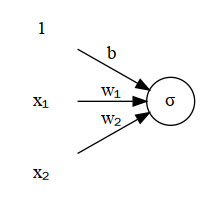
\includegraphics[width=0.4\textwidth]{./plots/neuron.gv.png}
%\label{fig:neuron1}
\end{subfigure}
\begin{subfigure}[b]{0.45\textwidth}
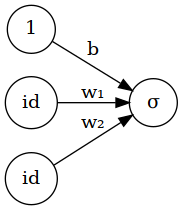
\includegraphics[width=0.4\textwidth]{./plots/neuron.2.gv.png}
\end{subfigure}
\caption{Two graphical descriptions of the neuron
$\sigma(w_1x_1 + w_2x_2 + b)$}. Here the bias $b$ is explicitly shown
but usually it is not depicted. In the left the variable names are explicitly
shown, while in the right they are not.
\label{fig:neuron2}
%\end{framed}
\end{figure}

Connecting many neurons together can create powerful parameterized
functions which we call neural networks.
%Connecting means that the output of one neuron is the input to one of the
%variables of a different neuron.
In feed forward networks the information only goes in one direction (no
feedback) and as we will see it means the network is a directed acyclic graph.

\begin{mydef}
\label{def:NN}
A \emph{feed forward neural network (NN)}is a \textbf{parameterized} map $\phi$
recursively defined
follows:
\begin{enumerate}
\item{} 
Activation functions ($1$, $id$, and $\sigma$) are NNs which are called the
\emph{elementary neurons} and they have no parameters ($\w=\emptyset$).
\item{} neurons are NNs
\item{} If $\psi :\R^n \to \R^m$ is a parameterized linear map then it is a NN.
\item{} If $\psi : R^n \to \R^m$
and $\rho: \R^m \to \R^l$ are NNs and their parameter sets are disjoint then $\phi = \rho
\circ \psi$ is a NN.
\item{} if $\nu:\R^n \to \R^m$ is a NN
and if $\psi_i: \R^{k_i} \to \R^{n_i}, i =1 \dots l$ are NNs, such that
$\sum_1^l n_i = n$
%and if $\psi_1, \dots \psi_n$ are NNs,
and if the parameter set of $\nu$ is disjoint from the combined parameters of
the $\psi_i$'s then
$\phi = \nu(\psi_1, \dots, \psi_n)$ is a NN
%if the dimensions "make sense".
.
\end{enumerate}

The parameter set $\w$ is called the \emph{weights} of $\phi$.
Often we don't distinguish between the network $\phi$ and its weights, and
we identify both as $\phi$.

In the definition we made the range and domain to be the entire $\R^n$ but
it is not necessary, we just need for the composition to be valid.
\end{mydef}

Feed forward neural network 
are depicted as a directed acyclic graph where every node (with its incoming
edges) corresponds to a neuron.
You can think of figure~\ref{fig:neuron2} left as depicting the neuron "component" 
in a network, while figure~\ref{fig:neuron2} right shows a neural network
description of single neuron, comprised from elementary neurons.

If rule 5 of the definition~\ref{def:NN} is not used in the construction of $\phi$, then the
resulting network is hierarchical. Its graph can be partitioned into \emph{levels}
$l_0, l_1\dots$ and there are only directed edges between two consecutive
levels $l_i \to l_{i+1}$ (see figure~\ref{fig:nn1}).

The label inside the neuron describes its activation function.
In the diagrams, we let $\sigma$ represent the sigmoid function.
We represent the identity function either by the name of the variable ($x_1$,
$y$ etc.) it acts on or simple by 
$id$.   We let the label $1$ represent the constant function. We need the
constant function because with it we can represent any affine map as a linear
map with the first input always clamped to $1$. But connecting $1$ to every
(non-input level) neuron would clutter the graph so it is not shown in most
diagrams but still implicitly assumed.
A directed edge between neurons means that the output of the neuron at the tail
is multiplied by the edge weight and assigned to the input variable of the
neuron it connects to.
A Node's output is therefore only dependent on the output of its direct
ancestral nodes 
(plus the bias which is usually not shown).
Input-level neurons (sources) have no incoming edges and they represent the
beginning of the
computation.
Output neurons (sinks) have no outgoing edges and their output is the final result of
the computation.


\begin{figure}[h]
%\begin{framed}
\centering
\begin{subfigure}[b]{0.5\textwidth}
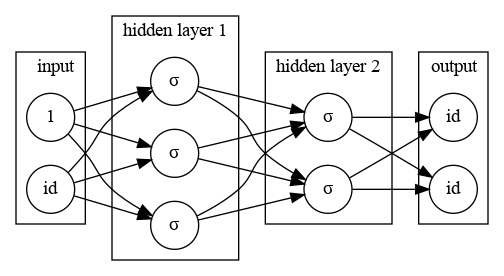
\includegraphics[width=0.8\textwidth]{./plots/neuronlayers.gv.png}
\end{subfigure}
\begin{subfigure}[b]{0.5\textwidth}
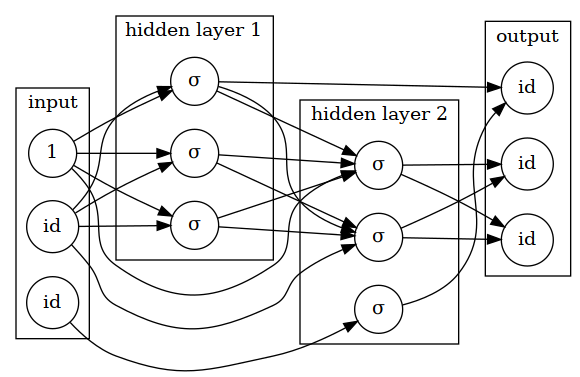
\includegraphics[width=0.8\textwidth]{./plots/neuronlayers.2.gv.png}
\end{subfigure}
\caption{The network in the top didn't use rule 5~\ref{def:NN} in the construction.
It is strictly hierarchical and there are only edges between nodes of two
consecutive layers. The one on the bottom is more general.
}
\label{fig:nn1}
%\end{framed}
\end{figure}

It turns out~\cite{nielsen2015neural} that the feed forward neural networks
with a single type of non-linear activation (e.g. sigmoid) and a single hidden
layer
are "universal"; Which means that
any continuous function $f$ can be
uniformly approximated by a feed forward neural network
with a single hidden layer and Sigmoid as the non-linear
activation function.
More precisely, let $B \subseteq \R^n$ be a bounded domain. Let $f : B \to \R^m$
be continuous, and let $\epsilon \in (0,1)$. Then there is a feed forward neural
network with a single hidden layer $\phi = \phi_{\w}$ and there is some value assignment
for the parameters $\w$ such that 
$(\forall \x \in B) \|\phi(\x) - f(\x)\|_2 \lt \epsilon $. The size of that single
hidden layer (the number of parameters) depends on $f$ and $\epsilon$.

In the definitions we only used linear maps to grow the network. 
There are other types of maps which are used, most commonly are convolutions 
but the principles and the graphical description remain essentially the same.

There are additional types of parameterized functions which are used "within the
layer" such as batch normalization but we won't get into that as this is not a
thesis about neural networks per se.

\begin{figure}[h]
%\begin{framed}
\centering
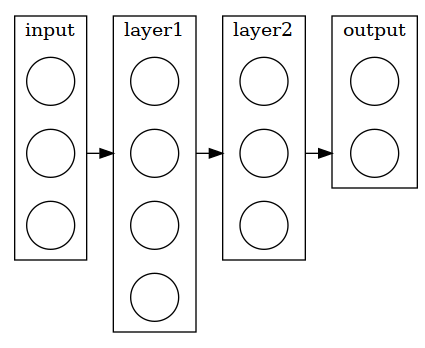
\includegraphics[width=0.5\textwidth]{./plots/multilayer.gv.png}
\caption{
A graph of a hierarchical feed forward neural network where the connections 
are abstracted. Edges between layers may represent in this case a fully
connected layer (every neuron has incoming edges from all neurons of the
previous layer) but it could also be used for describing a convolution.
}
\label{fig:nn2}
%\end{framed}
\end{figure}

As figure~\ref{fig:nn1} shows, 
The input layer is the where the input $(\x)$ is "fed in" and the output layer
is the final result of the evaluation $\phi(\x)$.
We call all the layers (or neurons) that are 
not in the input level or the output level "hidden"
because we don't usually know what is the input/output value in these.

\section{Loss functions}

In the claim about neural networks being "universal" in terms of approximating
function $f(\x)=\y$ with neural network $\phi(\x)$. We stated specifically
convergence in terms of $l_2$ norm
$\|\phi(\x) - \y \|_2$, but the claim holds in theory and in
practice with other types of "distance-like" functions which we call loss
functions.

Moreover we usually don't know what is the function $f$ which we try to
approximate. Rather we are given 
paired samples of input/target $(\x, \y)$ and we
try to minimize the total error.

\begin{mydef}
\label{def:lossfunc}
Let $\phi :\R^n \to \R^m$ be a neural network.
A \textit{loss function} is a differentiable
function $\mathcal{L} : \R^{m}\oplus\R^m \to \R$. 
With "distance-like quality".
\end{mydef}

Typically the loss function is additive on the dimension, meaning it has the
form $(\forall \y,\z \in \R^m) \mathcal{L}(\y, \z)) = \sum_{i=1}^m \psi(y_i,
z_i))$

Let $\X \in \R^{N \times n}, \Y \in \R^{N \times m}$ be the input and the target
set and let $(\x,\y)$ be a paired input/target. 
We use the loss function $\mathcal{L}$ as the target function for 
the minimization problem,
 $\min_{\w} \sum_{(\x,\y)}\mathcal{L}(\phi(\x), \y)$ where the sum goes over all
paires ($N$ rows)  (input, target).


For example
$\mathcal{L}(\y, \z)) = \|\y - \z\|_2^2 = 
\sum_i |y_i - z_i|^2$ is a one such loss function (the
square error).

So far we defined $\phi$ and $\mathcal{L}$ on single input/target data points
$\x$ and $\y$. But we are interested in minimizing the total error
$\mathcal{L}(\phi(\X),\Y)$. So first we need to state how these functions
operate on sets of samples (matrices) rather than on data points (vectors).

Usually evaluation over the entire dataset is infeasible. Instead computation is
performed on batches, which are relatively small chunks of the data.

\begin{mydef}
\label{def:batch}
Let $\bv{X} \in  \R^{N \times n}$ be a data matrix. A \emph{batch}
$\bv{x} \in \R^{b \times n}$ is any subset of $b$ rows of $\bv{X}$
(Note that in this case $\x$ represents a matrix).
\end{mydef}

Batch $\x = \{\x_1, \dots \x_b\} \in \R^{b \times n}$ (row notation)
represents a subset of $b$ samples out of the total of $N$ samples in the
dataset.
Extending $\phi$ to operate on batches is trivial.
$\phi(\x) = \{\phi(\x_i)\}$ is the matrix where $\phi$ is applied on the rows of
the batch.
Given an input batch $\x$ and corresponding target batch of $\y$,
We extend the loss function to batches by averaging over the batch:
$\mathcal{L}(\phi(\x), \y) \triangleq \frac{1}{b} 
\sum_{i=1}^b \mathcal{L}(\phi(\x_i), \y_i)
$

\begin{mydef}
Let $\phi$ be a neural network as defined in~\ref{def:NN} and let $\mathcal{L}$
its associated loss function as defined in~\ref{def:lossfunc}---over vectors.
Let $\x = \{\x_1, \dots , \x_b\} \in \R^{b \times n}$ be a $b$-batch (in row
notation)
, and let $\y = \{\y_1, \dots , \y_b\} \in \R^{b \times m}$ be a corresponding
target batch.
Then $\phi$ and $\mathcal{L}$ \emph{extended} over batches are:
\begin{IEEEeqnarray}{C}
\phi(\bv{x}) \triangleq \{\phi(\bv{x}_i)\}_{i=1}^b \in \R^{b \times m}\\
\label{eq:NNbatch}
\mathcal{L}(\phi(\x), \y) \triangleq \frac{1}{b}\sum_{i=1}^b \mathcal{L}(\phi(\x_i), \y_i) \in \R
\label{eq:NNbatchloss}
\end{IEEEeqnarray}
\end{mydef}

If $\mathcal{L}$ is the square error function $\| \cdot \|_2^2$ on vectors,
then its extension to batches is $\frac{1}{b}\| \cdot \|_F^2$. The reason why we
sum and don't average over the dimensions will be cleared later when we get into
variational inference.

There is also a probabilistic way to interpret the total loss.
We assume that the data points $\X, \Y$ were randomly and independently sampled from the unknown
data distribution $p(\x, \y)$.
Then equation~\ref{eq:NNbatchloss} can be reformulated as the expected 
loss~\cite{bishop2006pattern}:

\begin{equation}
\mathcal{L}(\phi(\X), \Y) \approx
\mathrm{E}_{\x,\y \sim P(\x,\y)} \mathcal{L}(\phi(\x), \y)
\label{eq:NNbatchlossE}
\end{equation}

\section{Training}
This is just a brief explanation of the basic principals. Training deep networks
is a big subject which has many challenges and obstacles and a lot of
heuristics are used. 

Training the neural network $\phi_w$ means finding the weights that minimize the
loss function applied on the training input/target paired sets $\X,\Y$, in other
words minimizing $\min_{w} (\mathcal{L}(\phi_w(\X),\Y)$.
Usually we can't compute efficiently $\phi$ and $\mathcal{L}$ over the entire
sets because $N$ is too large, therefore we use batches.

\begin{mydef}
Let $\phi_{\omega}$ be a neural network and $\mathcal{L}$ its associated loss
function. And let $(\X, \Y)$ be our \emph{training set} consisting of 
the data matrix $\X$ and $\Y$
the corresponding target matrix.
Then \emph{Training} of $\phi_{\omega}$ with respect to $\mathcal{L}, \X$ 
means
algorithmically approximating the minimization problem:
\begin{equation}
\label{def:training}
\min_{\omega} \mathcal{L}(\phi_{\omega}(\X), \Y)
\end{equation}
\end{mydef}

During a \emph{training step} the network is applied on a batch $(\x,\y)$. Then the
loss function is applied on the output of the network and a gradient (with relation to the
weights) is taken using the efficient backpropagation
algorithm~\cite{nielsen2015neural}.
The gradient is used for the weight update rule, which
varies depending on the specific training algorithm. Typical training algorithms
are SGD (stochastic gradient decent) and Adam~\cite{jais2019adam},
which is the one used throughout
this work.

We only need to define the network, the loss function and the specific training
algorithm. The rest (derivation, weight update etc.) is taken care for us by the
backend of the software (Pytorch~\cite{pytorch2018pytorch}) and can be regarded
as a black box.

\subsection{Training, validation and testing data sets}

The data is partitioned into disjoint sets. The training set is used for the
training of the model. The testing set is used for the final performance
assessment. Sometimes a third subset, the validation set is used for tuning and
tweaking the model during training. The point is that the model "doesn't know"
the validation data because the weights are only trained on the training set,
but the hyper-parameters are optimized based on the validation set.
For example the validation set can be used for early
stopping during the training.
We didn't use a validation subset in our tests.
Finally the assessment is performed on the 
testing set which was completely held out during the training and
hyper-parameter tuning.


\subsection{Un/Supervised learning}

In unsupervised learning one seeks to "learn" or infer the target set $\Y$ (for example
category information) from $\X$ without seeing $\Y$ during training.
For example in the case of MNIST we want to teach the model to distinguish
10 categories of images corresponding to the $10$ digits, without having access
to the digit tags in the training set.

Supervised learning means the $\Y$ target information is fully accessible (every image
is tagged with the digit it represents). This is a much simpler classification
task.

Semisupervised learning is the hybrid case of both, where the training set
includes a small portion of known paired input/targets $(\x,\y)$ while for the
rest of the training set we only have $\x$ input and need to infer $\y$.
Semisupervised learning tasks often arise in natural situations. For example
there may be a large image data set where only a portion of the images have been
manually tagged.

\section{Autoencoders}

The basic type of an autoencoder which we informally call "vanilla" autoencoder
is a neural network that tries to "learn" the identity function. Though it sounds
pointless on a first thought, the point is how we construct this network. An
autoencoder consists of two neural networks.
An encoder network maps the input into a lower dimensional so called "latent
space", and a decoder network maps the latent space back into the high
dimensional input layer.
In the case of the vanilla autoencoder the target for the loss function is the
same as the input $\Y = \X$.

\begin{figure}[h]
%\begin{framed}
\centering
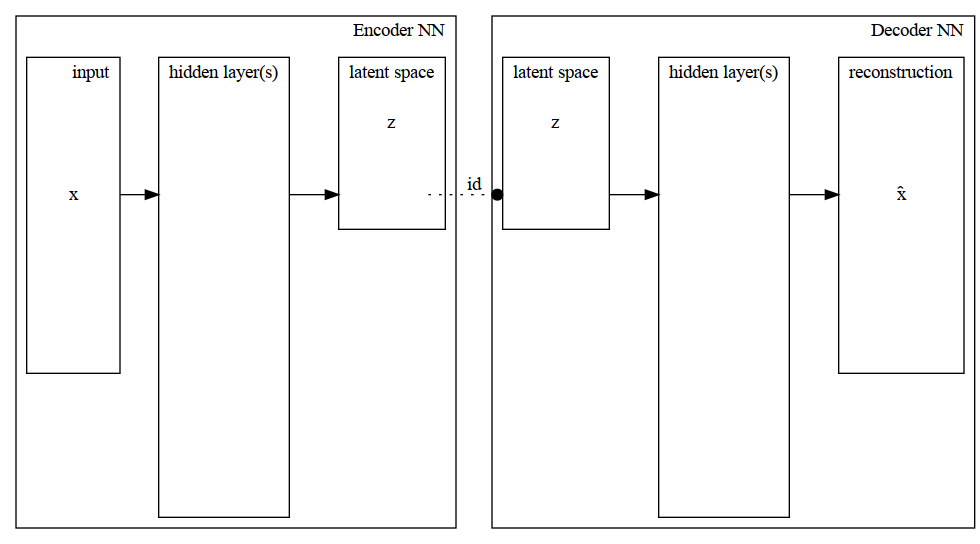
\includegraphics[width=0.8\textwidth]{./plots/autoencoderNN.gv.png}
\caption{
A graphic description of a "vanilla" autoencoder.
}
\label{fig:autoencoder}
%\end{framed}
\end{figure}

\begin{mydef}
\label{def:autoencoder}
An \textit{Autoencoder} (AE) is a pair 
$(\phi, \psi)$ of feed forward neural networks 
$\psi : \R^n \to \R^m, \nu : \R^m \to \R^n$.

$\psi$ is called the \emph{encoder} network, and $\nu$ is called the
\emph{decoder} network and the composition
$\phi = \nu \circ \psi$ is called the \emph{autoencoding network}. 

We call $\R^m$ or more genrally the domain of the decoder, \emph{the latent
space}, and $\R^n$ (or more generally the domain of the encoder) is called
\emph{the observed space}.

Given a batch $\x \in \R^{b \times n}$ we call $\z = \psi(\x) \in \R^{b \times m}$
the \emph{latent representation} of $\x$ or the \emph{encoding} of $\x$.
\end{mydef}

While the definition as is given is symmetric, it is assumed that $n > m$, and
therefore $\psi$ represents dimensional reduction (in other words encoding) of
the data and $\nu$ represents expansion back to original space (decoding).

The idea here is that the original high dimensional data can be embedded
in a low dimensional space by the encoder. The decoder then can reconstruct the
original data from the embedding.

There are many variations of autoencoders. For example a "denoising" autoencoder is
essentially that same model but it receives a "noisy" version of the input and
tries to reconstruct the original clean version.
We informally call the type of autoencoder of
definition~\ref{def:autoencoder} which aims to learn the identity function 
on the original input, and which is using the square error loss function, 
a "vanilla" autoencoder. 

\subsection{Relation between PCA and AE}
For \textbf{centered} data, where every variable (column of $\bv{X}$)
has a sample mean of $0$, the first $k \leq \text{rank}(\bv{X})$ principle components
$\bv{P}$ are the solution for equation~\ref{eqn:pca}; Whereas a \textbf{linear}
autoencoder solves equation~\ref{eqn:pca3}. As mentioned, it must hold that $E =
D^{\dagger}$ (the encoder must be the Moore-Penrose inverse of the decoder).

A linear autoencoder with the  square error
loss function is almost equivalent to
PCA~\cite{plaut2018principal}; At the optimum, a bottleneck space of dimension $k$
is spanned by the first $k$ principle components of the input $\bv{X}$.
In general, an AE can be seen a PCA-like, but non-linear method for
dimensionality reduction.

\begin{figure}[h]
%\begin{framed}
\centering
\begin{subfigure}[t]{0.45\textwidth}
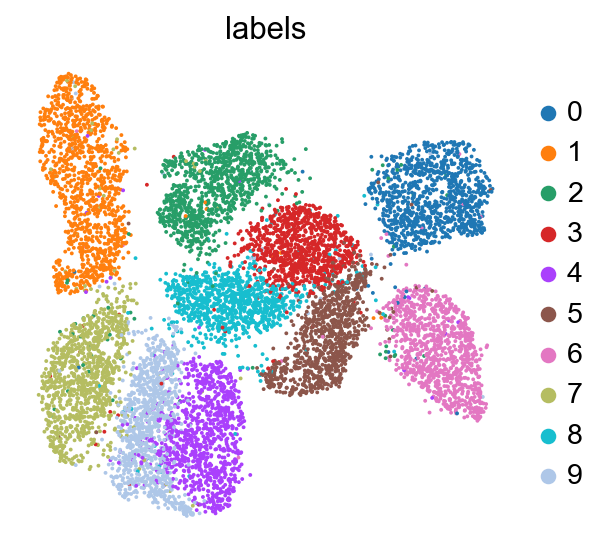
\includegraphics[width=0.95\textwidth]{images/pca.umap.mnist.png}
\caption{MNIST: UMAP of the PCA}
\end{subfigure}
\begin{subfigure}[t]{0.45\textwidth}
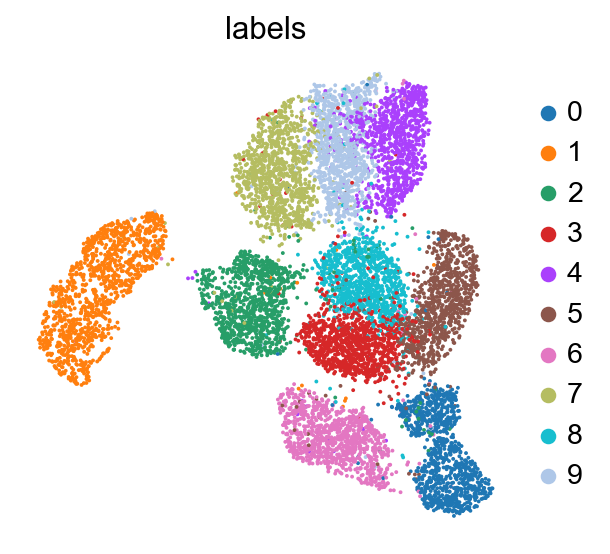
\includegraphics[width=0.95\textwidth]{images/ae.umap.mnist.png}
\caption{MNIST: UMAP of the AE}
\end{subfigure}
%\end{framed}
\caption{PCA (l) compared with "vanilla" autoencoder (r) on the MNIST dataset}
\label{fig:pcavae}
\end{figure}

Figure~\ref{fig:pcavae} shows on the left a
UMAP~\cite{mcinnes2018umap} of the principle components of the testing subset of
MNIST (images of hand written digits). On the left we see a UMAP of the latent
space encoded by the encoder of a "vanilla" autoencoder with the square error loss
function. The autoencoder was
trained on the training set and didn't "see" the testing images during training.
The results appear quite similar.

\chapter{Variational inference and variational autoencoders}
\section{Variational Inference}

Here we briefly explain the idea behind variational inference and introduce the
ELBO which is the loss function we'll use throughout this text.
For more details see~\cite{bishop2006pattern}.

We treat the data matrix as a set of independent observations (its rows)
$\bv{X} = \{\bv{x}_1, \dots
, \bv{x}_N\}$ which we try to explain by a probabilistic model. 
Each row $\x_i$ is considered a realization of a random vector, which we also 
denote by $\x_i$ (as explained in the notation section) and similarly $\X$
represents both the set of r.vs as well as the realization.

We assume that
the $\bv{x}_i$'s are independent and identically distributes (i.i.d) random vectors
with some distribution function $\x \sim p(\x)$ and therefore for
the entire dataset it holds that $p(\bv{X}) = \prod p(\bv{x}_i)$.

\begin{mydef}
\label{def:logevidence}
Let $\bv{X} \in \R^{N \times n}$ be a data matrix and let $\{\bv{x}_i\}_1^n$ be its
rows,
which we assume to be i.i.d with some (unknown) distribution $\x \sim p(\bv{x})$.
Then $\log p(\bv{X}) = \sum_1^N \log p(\bv{x}_i)$ is called the \emph{log evidence} of our
data.

$\frac{1}{N}\log p(\X)$ is the \emph{mean log evidence} (remember the
mean-sum rule for data sets and
batches~\ref{meansumrule}).
\end{mydef}

An observation r.v $\bv{x}$ is high dimensional however
we have some reason to believe that behind the scenes there is some hidden
(latent), smaller dimensional random vector $\z$ that generates it.
In other words we think that $\x$ is conditioned on $\z$ and we can speak of
the joint distribution $p(\x,\z) = p(\x | \z)p(\z)$.
And again $\x_i$ only depends on $\z_i$ so everything factors nicely, e.g. 
$p(\X | \Z) = \prod_i p(\x_i | \z_i)$.

Suppose that we have a fully Bayesian model. In this case there are no
parameters because the parameters are themselves stochastic variables with some
suitable priors. We can therefore pack all the latent variables and stochastic
parameters into one latent "meta variable" $\z$,
which is some multidimensional r.v and which is possibly composed of several simpler r.vs (for
example a categorical and a normal r.vs).
We similarly pack all the observed variables into one meta variable $\bv{x}$.
Together we have a distribution $p(\bv{x},\bv{z})$ and the working assumption is that it
is easy to factorize $p(\bv{x},\bv{z}) = p(\bv{x}|\bv{z})p(\bv{z})$,
however $p(\bv{z}|\bv{x})$ is intractable and
$p(\bv{x})$ is unknown.

We are being Bayesian here so we consider $\bv{X} = \{\bv{x}_1, \bv{x}_2, \dots
\}$ to be
a constant set of observations and we want to best explain $p(\bv{X})$ by finding as
high as possible lower bound for it (or rather to $\log p(\bv{X})$, the \emph{log
evidence}).
A second goal is to approximate the intractable $p(\bv{z}|\bv{x})$ by some simpler
distribution $q(\bv{z})$ taken from some family of distributions.

\begin{mydef}
Let $\bv{x},\bv{z}$ be random variables with joint
distribution $p(\bv{x},\bv{z})$ and let $q(\bv{z})$ be any distribution.
Let $(\X,\Z) = \{(\x_1,\z_1), \dots , (\x_N,\z_N)\}$
be $N$ independent replications of $(\x,\z)$.
The \emph{evidence lower bound (ELBO)} with respect to $p,q$ is:
\begin{IEEEeqnarray}{C}
\label{def:elbo}
-\mathcal{L}(q,p,\x) \triangleq
\int \log \frac{p(\bv{x},\bv{z})}{q(\bv{z})} d q(\bv{z}) \\
\label{def:elboX}
-\LL(q,p) \triangleq 
-\LL(q,p, \X) 
= \frac{1}{N} \sum_1^N (-\LL(q,p,\x_i) \\ 
\approx
\E_{\x} [-\LL (q,p, \x)]
\end{IEEEeqnarray}
\end{mydef}

Equation~\ref{def:elboX} is no longer treated as a function of $\X$ because it
is taken over all of our data which we think of as a constant.
The reason that we mark the ELBO with $-\LL$ is because we use the minus ELBO,
$\LL$, as the 
loss function for VAEs.

The following equation shows that the \emph{ELBO} is a lower bound for the
\emph{mean log
evidence}.
(using Jensen's inequality)

\begin{equation}
\label{eq:elbo}
\begin{aligned}
\frac{1}{N} \log p(\bv{X}) &= \frac{1}{N} \log \int p(\bv{X},\bv{Z}) d\bv{Z} 
= \frac{1}{N} \log \int \frac{p(\bv{X},\bv{Z})}{q(\bv{Z})} q(\bv{Z})d\bv{Z} \\
&=  \frac{1}{N} \log \int \frac{p(\bv{X},\bv{Z})}{q(\bv{Z})}dq(\bv{Z}) 
\geq  \frac{1}{N} \int \log \frac{p(\bv{X},\bv{Z})}{q(\bv{Z})}dq(\bv{Z}) \\
&= \frac{1}{N} \int \sum_1^N \log \frac{p(\x_i, \z_i)}{q(\z_i)}dq(\z_i) \\
&= \frac{1}{N} \sum_1^N - \LL(q,p,\x_i)
= -\mathcal{L}(q,p,X) \triangleq -\mathcal{L}(q,p)
\end{aligned}
\end{equation}

In equation~\ref{eq:elbo} we found a lower bound $-\mathcal{L}(q,p)$ for the
mean log
evidence $\log p(\bv{X})/N$, the \emph{ELBO}.
Whatever distribution $q$ we put in ELBO will not be
greater than the real log evidence so we are looking for the $q$ which
\textbf{maximizes} it.

Now we show that maximizing the ELBO actually obtains the mean log evidence and it is
equivalent to minimizing $KL(q(\bv{Z}) \| p(\bv{Z}|\bv{X})$:

\begin{equation}\label{eq:kl_bound}
\begin{aligned}
-\mathcal{L}(q,p,\x) &\triangleq \int \log \frac{p(\bv{x},\bv{z})}{q(\bv{z})} d
q(\bv{z})
= \int \log \frac{p(\bv{z}|\bv{x})p(\bv{x})}{q(\bv{z})} d q(\bv{z}) \\
&= \int \log p(\bv{x}) dq(\bv{z}) - \int \log \frac{q(\bv{z})}{p(\bv{z}|\bv{x})}
dq(\bv{z}) 
= \log p(\bv{x}) - KL(q(\bv{z}) \| p(\bv{z}|\bv{x})
\end{aligned}
\end{equation}

We can rewrite equation~\ref{eq:kl_bound} as:
\begin{equation}\label{eq:elbokl}
\log p(\bv{x}) = -\mathcal{L}(q,p,\x) - KL(q(\bv{z}) \| p(\bv{z}|\bv{x}))
\end{equation}

Equation~\ref{eq:elbokl} shows that the ELBO minus the kl-divergence are constant
and equal the log evidence. Therefore minimizing the kl-divergence (which is
always non-negative) simultaneously maximizes the ELBO and vicer-versa.

\section{Variational Autoencoder}
\subsection{Adding parameters}

Our models will not be fully Bayesian, but rather parametrized.
Suppose that the $p$ distribution over $\x,\z$ belongs to some parametrized family of
distributions $p_{\theta}(\x)$ and the $q$ distribution over $\z$ belongs to another
family $q_{\phi}(\z)$. In a fully Bayesian model we would make $\theta$ and
$\phi$ stochastic parameters and give them appropriate prior distributions, but
with the VAE we leave them as parameters that we determine with neural network
as will shortly be explained.

For any $\theta$ and any $\phi$, the equations from the previous chapter hold
also in the parametrize form, i.e 
$\log p_{\theta}(\x) =
-\mathcal{L}(q_{\phi},p_{\theta},\x) -
KL(q_{\phi}(\z) \| p_{\theta}(\z|\x))$.

We assume that we can only approach the "real" distribution using
$\theta$ from below $\log p(\x) \geq \log p_{\theta}(\x)$.
So together with equation~\ref{eq:elbo} we have

\begin{equation}\label{eq:parelbo}
\begin{aligned}
(\forall \theta, \phi)\log p(\x) & \geq \log p_{\theta}(\x) 
\geq -\mathcal{L}(q_{\phi}.p_{\theta},\x)
= \int \frac{p_{\theta}(\x,\z)}{q_{\phi}(\z)} dq_{\phi}(\z)
\end{aligned}
\end{equation}

And from equation~\ref{eq:elbokl} we again see that by finding the parameters
$\phi$, $\theta$ that maximize the ELBO we approach the real log evidence as much
as we can within the limits of the parametrized family of distributions we use.

\subsection{Rearranging the ELBO}
Equations~\ref{eq:elbo} and~\ref{eq:kl_bound} were defined for any distribution
$q(\z)$ and in particular we are allowed to plug in a conditioned
distribution $q(\z|\x)$. That implies the existence of $q(\z,\x)$ and $q(\x)$
but we actually don't care about them. We condition everything on $\x$ but $\x$
is treated as a given constant from a Bayesian view point and we only want to
somehow make $q(\z|\x)$ to closely approximate $p(\z | \x)$.

A second thing we need to achieve is to express the -ELBO in terms of $p(\x|\z)$
and $q(\z|\x)$ rather than the joint distribution. To that end we need also the
prior $p(\z)$.

%\begin{mydef}
%The \emph{conditioned (on $\X$) ELBO} is
\begin{equation}
\begin{aligned}
\mathcal{L}(q,p,\x) &\triangleq \int -\log \frac{p(\x,\z)}{q(\z|\x)}dq(\z|\x) 
= \int -\log \frac{p(\x |\z) p(\z)}{q(\z|\x)}dq(\z|\x) \\
&= \int -\log p(\x | \z)dq(\z|\x) + \int \log \frac{q(\z|\x)}{p(\z)}dq(\z|\x) \\
&= \int -\log p(\x | \z)dq(\z|\x) + KL(q(\z|\x) \| p(\z))
\label{eq:elbo_conditioned}
\end{aligned}
\end{equation}
%\end{mydef}

So to sum it up, if we want to maximize the log evidence $\log p(\X)$ it
suffices to minimize $\mathcal{L}(q,p)$ and equation~\ref{eq:elbo_conditioned}
shows that this means finding the balance between making 
the term $\int \log p(\X | \Z)dq(\Z|\X)$ (which we call the reconstruction term) large as possible, 
and making the KL-term small.
The KL term is seen as a regularization term.

\subsection{Using neural networks for the parametrization}
In this text we deal with variational autoencoders (VAE).
A VAE is a neural network which is used to define and optimize the parameters
$\phi$ and $\theta$ which define $p_{\theta}(\x | \z)$ and $q_{\phi}(\z | \x)$
and we train the network to maximize equation~\ref{eq:elbo_conditioned}.

Specifically the encoder part of the network is a feed forward neural network 
$f_{\theta}(\z)$ which is
used to define the distribution $p_{\theta}(x|z)$. For example, we can assume that $p_{\theta}$
is a family of multivariate Gaussians and in this case $f_{\theta}(z) =
(\mu(z), \Sigma(z))$. Meaning the encoder maps $z$ to the location vector and
covariance matrix. The parameter $\theta$ in this case are the weights of the
encoder neural network. 

The decoder network is similarly defined as neural network $g_{\phi}(\x)$ which
maps $\x$ into the parameters defining the family $q_{\phi}(\z)$. Here too $\phi$
represent the weights of the decoder.

For the prior $p(\z)$ we set some fixed prior distribution.

Note that the encoder network (similarly the decoder) is used to define a distribution over
$\z \in \R^m$, but the encoder itself maps into some other space. 
For example,
to define a normal one Gaussian distribution (so over $\z \in \R$, the encoder
maps into $\R^2$, and its output creates $\mu, \sigma \R$ which are used to
define the Gaussian distribution $\mathcal{N}(\z ; \mu, \sigma)$.
We also need to make sure that the range of the network obeys to the constraints
of the parameters. For example the variance must be non-negative. 
Alternatively we can use transformations to remove constraints. For example
instead of letting the network specify the variance. we let it specify the
log-variance.

\begin{mydef}
\label{def:vae}
Let $\{p_{\theta}\}_{\theta \in \Theta}$ be a parameterized 
family of distributions over $\R^n$ and let
$\{q_{\phi}\}_{\phi \in \Phi}$ be a family of distributions over $\R^m$.
Where $\Theta$ and $\Phi$ are real domains (i.e $\Theta \subseteq \R^k \dots$).

A \emph{variational autoencoder (VAE)} consists of a pair $(E,D)$ of neural networks,
$E : \R^n \to \Phi$ and $D : \R^m \to \Theta$ and some fixed distribution $p \in
\Phi$.

We call $\R^m$ or more genrally the distribution space of the decoder, \emph{the latent
space}, and $\R^n$ (or more generally the distribution space of the encoder) is called
\emph{the observed space}.
$p$ is called \emph{the prior distribution of the latent space}.
\end{mydef}

An autoencoder works deterministically, where 
the encoder maps the input $\x \mapsto \z$ and the decoder then maps the
latent space $\z \mapsto \hat{\x}$ to the reconstruction. A VAE does
basically the same thing but non-deterministically.
It maps $\x$ into a distribution over $\z$: $\x \mapsto q(\z|\x) =
q_{\phi(\x)}(\z)$ and it maps
$\z$ into a distribution over $\x$: $\z \mapsto p(\x|\z) = p_{\theta(\z)}(\x)$.

The loss function associated with a VAE is minus ELBO. This means training
the VAE maximizes equation~\ref{eq:elbo_conditioned} and therefore also
the log evidence.

To give a concrete example lets say that the distribution family for $q_{\phi}$ 
is the diagonal normal distribution.
We can set the parameter domains $\Phi = \R^m \oplus \R^m$. The means can be any
real vector, but the variances are non-negative. We can either restrict the
encoder to be non-negative on the variance-domain, or we can agree to use the
log-variance as the second parameter, which is then unconstrained.

We identify $q(\z | \x)$ with the encoder but technically what it means is that 
the encoder network maps $\x$ into the distribution parameters $E(\x) = \phi(\x)
\in \Phi$;
in the case we use diagonal normal distribution $\phi(\x) = (\mu(\x), \sigma(\x))$
. Thus we defined a distribution over $\z$ by using $\x$ to map into
the parameter domain: $q(\z | \x) = q_{\phi(\x)}(\z)$

Similarly we call $p(\x | \z)$ the decoder although it is
technically the distribution defined by the decoder. $D(\z) = \theta(\z)$:
$p(\x | \z) = p_{\theta}(\x)$


\subsection{Mean field approximation}
Usually we treat the dimensions of $\x$, $\z$ etc. as independent.
That means if $\x = (x_1, \dots, x_n)$ is a r.v. in $\R^n$ 
we assume that the $x_i$ are independent and therefore 
$P(\x) = \prod_1^n p_i(x_i)$.

Specifically the mean fields approximation of a multivariate Gaussian
$\NN(\x | \bv{\mu}, \bv{\Sigma})$ is a diagonal Gaussian 
distribution 
$\NN(\x | \bv{\mu}, \bv{\sigma})
\triangleq \NN(\x | \bv{\mu}, \bv{\sigma}\bv{I})$.
Mean field approximation simplifies the implementation and speeds up the
computation and has been the standard practice since the
beginning of VAEs~\cite{kingma2013auto}.


\subsection{Computing the ELBO}
It may not be immediately clear how to how to compute the integral in the ELBO function. 
Recall that given an input $\x \in \R^n$,
The loss function is 

\begin{equation}
\LL(p,q,\x) = 
\int - \log \frac{p(\x|\z)p(\z)}{q(\z|\x)}dq(\z|\x)
= \int -\log p(\x|\z)dq(\z|\x) + \int \log \frac{q(\z|\x)}{p(\z)}dq(\z|\x)
\label{eq:elbovae}
\end{equation}

Given concrete input $\x \in \R^n$,
the decoder specifies a distribution over
$\z \in \R^m$ rather then a concrete deterministic point:
$\z \sim q(\z | \x)$. Suppose that we draw one concrete sample $\z \in \R^m$
taken from that distribution. Now that we have the concrete input $\x$ and a 
concrete $\z$ we can compute $\log q (\z | \x)$ as well as the prior $p(z)$.
Remember that the decoder takes $\z$ and produces a distribution $p(\x | \z)$.
With a concrete $\z$, and $\x$ we can also compute $\log p(\x | \z)$
So once we draw a specific sample $\z$ we can compute everything inside the
integral.

In fact what we have done is already a form of Monte Carlo integration.
More generally, instead of drawing just one concrete sample $\z$, we draw $k$ samples
$\z_i \sim q(\z | \x)$ per input $\x$, and take the average. Then we have

\begin{equation}
\begin{aligned}
\LL(p,q,\x) = 
\int - \log \frac{p(\x|\z)p(\z)}{q(\z|\x)}dq(\z|\x) \\
= \int -\log p(\x|\z)dq(\z|\x) + 
\int \log \frac{q(\z|\x)}{p(\z)}dq(\z|\x) \\
\approx \frac{1}{k} \sum_{i=1}^k [-\log p(\x|\z_i)
+ \log \frac{q(\z_i|\x)}{p(\z_i)} ]
\label{eq:elbomc}
\end{aligned}
\end{equation}

In practice we take just one ($k=1$) sample $z$ for each input data point $x$.
Remember that we are working on batches and computing an average loss over
batches so for a given batch we are taking many samples $\z$.
Experimental data shows that taking larger samples usually brings little
benefit~\cite{kingma2019introduction}.

\subsubsection{Reparameterization trick}

The loss function is computed by using Monte Carlo integration, which requires
taking samples $\z \sim q(\z | \z)$. But the loss function needs to be 
differentiable with respect to the model's parameters which are 
the encoder's weights $\phi$ and the
decoder's weights $\theta$. There is a method, "the reparameterization
trick" which uses
some random noise  which allows to express the
sample $\z = h_{\phi}(\epsilon, \x)$ as a deterministic smooth function of 
the parameters 
given random noise $\epsilon$~\cite{kingma2013auto}.

For example in the "vanilla" VAE, $\z$ is sampled from
diagonal Gaussian distribution $\phi(\x) = (\mu(\x), \sigma(\x))$. Sampling
$\z \sim \NN(\mu(\x), \sigma(\x))$ is equivalent to sampling standard
normal noise
$\epsilon \sim \NN(0,1)$ and taking $\z = \mu(\x) + \sigma(\x) \cdot \epsilon$.
Most other types of distributions (Dirichlet, Negative Binomial, etc.) can be
sampled using the reparameterization trick as deterministic, differentiable
transformation of Gaussian or uniform random noise and in Pytorch, this feature
is built into the distribution object types.


\subsection{Using the decoder for data generation}

Suppose that we have a vanilla auto encoder $(\phi, \psi)$ and suppose that we
want to generate synthetic data set that looks similar to the original data.
We need to choose points $\z \in \R^m$ from the latent space and project back to
observed space $\psi(\z) \in \R^n$. The question is then how to sample these $\z$?
It's not immediately clear how to do this because we don't know what is the
distribution in the latent space.

If we use a VAE instead, we know that $\z$ should have a distribution that is pretty
close to the prior $p(\z)$, which we can easily sample from.
Given a VAE $(E, D, p)$, synthetic data samples can be generated as follows:
sample $\z \sim p(\z)$. Then given the samples in the latent space, sample
from the decoder distribution $\x \sim D(\z)$, in the observed space.
Figure~\ref{fig:vaegen} shows randomly generated digits which were created in such 
process.

\subsection{Encoding data in the latest space with a VAE}

Unlike a vanilla autoencoder, a VAE doesn't deterministically encode input $\x$
but rather maps it to a distribution $q(\z | \x)$.
We can use the distribution's mean $\mu(\x)$ as the
encoding. 
Given observation $\x$, we can deterministically encode $\x$ into 
the latent space by taking the mean: $\x \mapsto \E [E(\x)]$. 
Since $q(\x | \z)$ is some kind of parameterized distribution for example 
$\NN(\z: \mu(\x), \sigma(\x))$  
the mean is a known parameter of the distribution so we don't need to estimate
it. See for example in figure~\ref{fig:vaeumapmeans}.

Alternatively we can deliberately add stockanticity to the encoding by 
non-deterministically drawing $\z \sim q(\z | \x)$ from the encoder
distribution,
as is dones in figure~\ref{fig:vaeumapsamples}.

\begin{figure}[h]
%\begin{framed}
\centering
\begin{subfigure}[t]{0.3\textwidth}
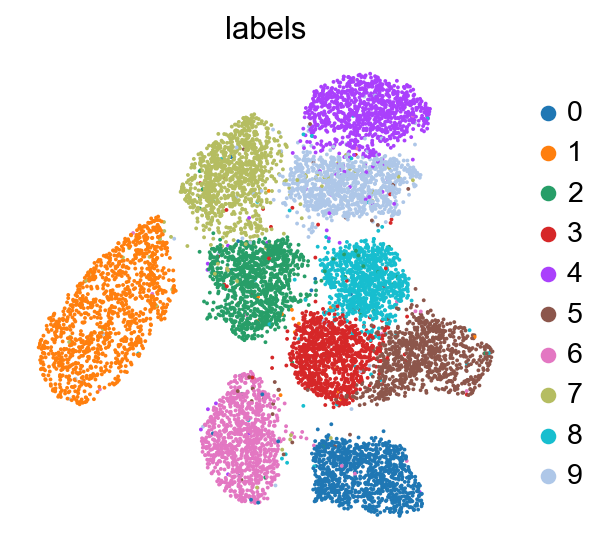
\includegraphics[width=\textwidth]{images/vae.umap.mnist.mu.png}
\caption{umap: means}
\label{fig:vaeumapmeans}
\end{subfigure}
\begin{subfigure}[t]{0.3\textwidth}
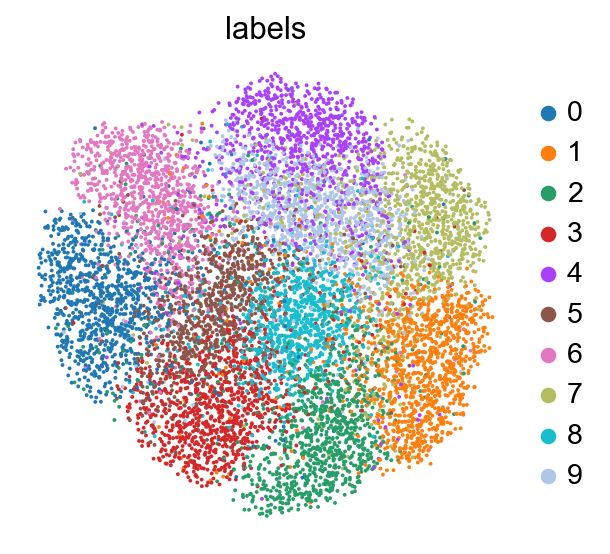
\includegraphics[width=\textwidth]{images/vae.umap.mnist.sampling.png}
\caption{umap: sampling}
\label{fig:vaeumapsamples}
\end{subfigure}
\begin{subfigure}[t]{0.3\textwidth}
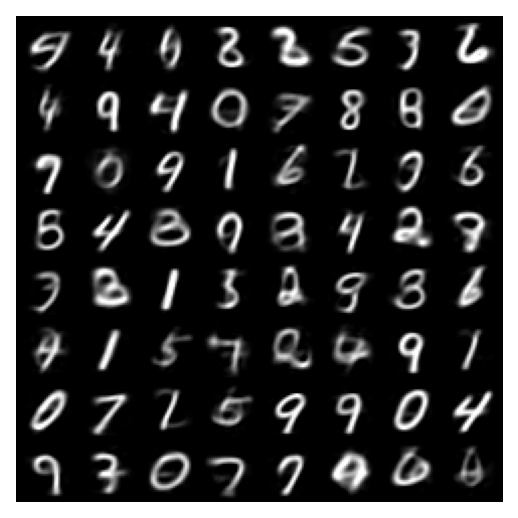
\includegraphics[width=0.9\textwidth]{images/vae.generation.mnist.sampling.png}
\caption{randomly generated digits}
\label{fig:vaegen}
\end{subfigure}
\caption{"vanilla" VAE trained on MNIST. The first two images show 
UMAP plot of the latent space $\z$.
In (a) we take the mean of the distribution $p(\z | \x)$ while in (b)
a random sample from the distribution is used.
Third plot shows random digits generated by sampling $z \sim p(\z | \x)$
and projecting back to the observed space $\x$ by the decoder.}
\label{fig:vaeumap}
%\end{framed}
\end{figure}


\subsection{Choosing the distribution types}
This is another topic that can get arbitrarily complex.

Recall that our loss function in the case that we take just one sample $\z$ for input $\x$
is:
\begin{equation}
\label{eq:vanillavaeloss}
\begin{aligned}
\LL(p,q,\x) 
= (-\int \log p (\x | \z)dq) + KL(q(\z | \x) \| p(\z)) \\
\approx -\log p (\x | \z) + \log \frac{\log q(\z | \x)}{p(\z)}
\end{aligned}
\end{equation}

The left term is called the reconstruction error and the 
right term is called the regularization term or the kl-term.


Lets suppose that we just want to use diagonal Gaussian distributions (which is
a type of mean field approximation).
The advantage is that it is easy to compute them because we just sum over the
dimensions:

\begin{equation}
\label{eq:diagnormal}
\log \NN(\x ; \bv{\mu}, \bv{\sigma}) = 
\sum_1^n \log \NN(x_i ; \mu_i, \sigma_i)
\end{equation}

The dimension of the latent space is a significant hyper parameter of the VAE
model.
Since we sum over the dimensions rather than averaging,
the larger we let the dimension of the latent space $\z$ 
it can have an effect of upscaling the importance of the kl-term relative to the
reconstruction.
Moreover the dimension should also be appropriate in terms of the "real"
dimensionality of the data.

In the case of the vanilla VAE we choose $p(\z) = \NN(\z;0,1)$ (diagonal
Gaussian standard normal) for the prior and 
$q(\z | \x) = \NN(\z ; \bv{\mu}(\x), \bv{\sigma}(\x))$ for the encoder.
There is a closed form formula for KL-divergence between two diagonal Gaussians
so in this case we don't need to use Monte Carlo integration for the KL-term
(we show it in one dimensions and for $k$ dimension in the diagonal case
we sum over the dimensions:

\begin{equation}
\label{eq:kldivnormal}
KL(\NN(;\mu_1, \sigma_1) \| \NN(;\mu_2, \sigma_2)) = 
-\frac{1}{2} + \log \frac{\sigma_2}{\sigma_1}
+ \frac{\sigma_1^2 + (\mu_1 - \mu_2)^2}{2 \sigma_2^2}
\end{equation}

The reconstruction term is more tricky.
Lets say we still want some sort of Gaussian diagonal distribution for $\x$,
so $p(\x | \z) = \NN(\x ; \bv{\mu}(\z), \bv{\sigma}(\z))$.
If we allow the decoder to create arbitrarily small variances, then the
decoder will stop being stochastic and it becomes deterministic. 
The decoder will also be able to pinpoint the sources in the latent space.
As a result the encoding becomes meaning-less and the encoded data will tend to
be arbitrarily spread in the latent space without meaningful clusters.
In addition there is a problem of numerical instability because the distribution
function can become arbitrarily large and the reconstruction loss might approach
$-\infty$.

A common approach is to use a fixed variance of $1$, because then the
reconstruction term becomes square error loss.
$p(\x | \z) = \NN(\x ; \bv{\mu}(\z), 1))$.

Another approach, $\sigma$-VAE~\cite{rybkin2021simple}, is to let the variance
be a trainable parameter but not a function of $\z$.
$p(\x | \z) = \NN(\x ; \bv{\mu}(\z), \bv{\sigma})$.
In this case as well in my experiments at least, if $\sigma$ is allowed to be
too small we sometimes get similar issues of numerical stability, 
non-stochastic decoder and meaningless 
encoding in the latent
space.

\subsection{VAE as a generalization of AE}
Suppose that we take a $\sigma$-VAE as described above, and suppose that we hold
$\sigma$ fixed.

So the decoder is $p(\x | \z) = \NN(\x ; \mu(\z), \sigma)$ where $\mu(z)$ is a a
function of $\z$ the decoder neural network. The decoder is $q(\z | \x) = \NN(\z
; \mu(\x), \sigma(\x))$ For the kl-term we use the analytical solution and for
the reconstruction error we use Monte Carlo integration with one sample. We can
assume that the KL term is uniformly (with respect to $\x$) bounded by some
constant $M$. We could also make sure that the encoder map is bounded but
normally there is no reason for the encoder to take the mean or the variance to
infinity during training as it would just increase the loss.

Our -ELBO loss function is:
\begin{equation}
\begin{aligned}
\LL(p,q, \x) = -\log \NN(\x; \mu(\z), \sigma) + KL(q(\z | \x) \| p(\z)) \\
= \frac{1}{2}\|\frac{x - \mu(\z)}{\sigma}\|^2 + \log \sigma + KL(q(\z | \x) \| p(\z))
\end{aligned}
\label{eq:losss}
\end{equation}

Minimizing $\LL(p,q,\x)$ in equation~\ref{eq:losss} is equivalent to minimizing 
$\sigma \LL(p,q,\x)$, and if we let $\sigma \to 0$ we get:
\begin{equation}
\begin{aligned}
\lim_{\sigma \rightarrow 0} \LL(p,q, \x) \sigma 
= \lim_{\sigma \to 0}[ -\log \NN(\x; \mu(\z), \sigma) \sigma + \sigma KL(q(\z |
\x) \| p(\z))] \\
= \lim_{\sigma \to 0} [\frac{1}{2}\|x - \mu(\z)\|^2 + \sigma \log \sigma  +
\sigma KL(q(\z | \x) \| p(\z))] = 
\frac{1}{2}\|x - \mu(\z)\|^2
\end{aligned}
\label{eq:lossss}
\end{equation}

So if we set $\sigma$ be arbitrary small, $p(\x | \z)$ become almost point mass
and the KL term loses significance, effectively removing the constraint from the
encoder. As a result the encoder itself
will also become point mass in order to minimize the reconstruction term and
disregarding the constraint on its distribution.
Thus the VAE becomes essentially a vanilla auto encoder at the limit.

\subsection{Graphical representation}
\label{sseq:graphical_representation}

It is both convenient as well as informative to include a graphical description
of our probabilistic models by way of modified plate diagrams which describes
both the generative model ($p$ distribution) and the inference model ($q$) on
the same graph.

\begin{mydef}
\label{def:platediagram}
A \emph{modified plate diagram} describes the factorization of two probabilistic
models with respectively
distributions $p$ and $q$, according to the following scheme.

\emph{Round or oval} nodes represent \emph{random variables}, \emph{rectangular
or square} nodes represent \emph{hyperparameters} or stochastic parameters,
and \emph{arrows} represent
dependency.

\emph{Solid arrows with pointed arrowhead} represent the dependencies of the $p$
distribution. \emph{Dotted arrows with round arrowheads} represent the dependencies of
the $q$ distribution.
In order to describe a legal distribution the subgraph of just the pointed
(and of just round) arrows must form a DAG.

Plate represents the packing of $N$ i.i.d random vectors.

Shaded nodes represent known values.
Shaded oval or round nodes are called \emph{observations} or \emph{observed
variables}.
Clear oval nodes are called \emph{latent} variables. 

Shaded square or rectangular nodes represent fixed hyperparameters of the model.
Clear square or rectangular nodes represent stochastic parameters of the model.
\end{mydef}

Figure~\ref{fig:vae_model} is a modified plate diagram of the VAE model.
We use doted arrows with round arrowhead to represent the inference model
(encoder network),
and regular arrows for the generative model (decoder network) so the combined
diagram describes the two networks together.

The squared $\zeta$ node represent some \emph{fixed hyperparameter} which describes the
prior distribution of $p(\z) := p(\z | \zeta)$.
It is possible to make $\zeta$ a non-fixed stochastic parameter but in the case of this
vanilla VAE I don't think it has any advantage and don't know of anyone who 
does that. 

The generative model therefore factors as: $p(\x,\z) = p(\x|\z)p(\z|\zeta) =
p(\x|\z)p(\z)$.
The inference model in this case is just $q(\z | \x)$.

\begin{figure}[h]
%\begin{framed}
\centering
\begin{subfigure}[b]{0.2\textwidth}
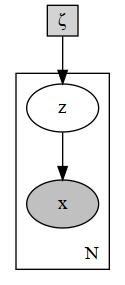
\includegraphics[width=\textwidth]{plots/vae_p.gv.png}
\caption{generative model ($p(x,z)$}
\end{subfigure}
\begin{subfigure}[b]{0.2\textwidth}
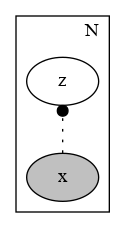
\includegraphics[width=\textwidth]{plots/vae_q.gv.png}
\caption{inference model ($q(z|x)$)}
\end{subfigure}
\begin{subfigure}[b]{0.2\textwidth}
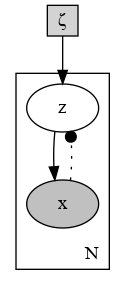
\includegraphics[width=\textwidth]{plots/vae.gv.png}
\caption{the combined graphical model}
\end{subfigure}
\caption{VAE graphical model}
\label{fig:vae_model}
%\end{framed}
\end{figure}

Note that the graphical model has no assumption about the specific types of
distributions involved (Gaussian, Dirichlet or whatever \dots) and that is left
for the actual implementation.

In the case of a "vanilla" VAE $(E,D,p)$, 
We use mean field approximation for $p$ and $q$ with Gaussian distributions.
We set the prior $p(\z)$ to be diagonal standard Gaussian
$p(\z) \sim \NN(;\bv{0},\bv{1})$.
And $p(\z | \x) \sim \NN(;D(\z))$ is a diagonal Gaussian, where the decoder
determines its means and variances $D(\z) = (\bv{\mu}(\z), \bv{\sigma}(\z))$, 
And similarly $q(\z | \x) \sim \NN(;E(\x))$.

%\begin{mydef}
%\end{mydef}


\section{Expanding the VAE model}
If we look at figure~\ref{fig:vae_model} it looks very simple, but it also
pretty much forces us to choose a simple type of distribution family (e.g
diagonal Gaussians in the case of the vanilla VAE).
Recall that That $\z$ packs up all the latent variables and the stochastic
parameters and $\x$ packs up all the observed variables.

We can describe a more complex distribution by unpacking them and describe the
dependencies between them.
This is done in the following way:
\label{VAE-specs}
\begin{enumerate}
\item{} Define the set of observed random vectors $\x_1, \x_2, \dots \x_k$, and 
the set of latent random vectors and stochastic parameters $\z_1, \dots \z_l$.
\item{} Specify how to factor the generative model $p(\x_1,\dots, \x_k| \z_1
\dots , \z_l)$
\item{} Specify how to factor the inference model $q(\z_1 \dots \z_l | \x1,
\dots \x_k)$
\item{} Choose appropriate priors $p(\z_i)$ and
\item{} Choose appropriate distribution families for the $\x_i$ and $\z_i$,
and choose priors $p(\z_i)$.
\end{enumerate}

\subsection{Example: CVAE}
Suppose that we have data that carries both numerical and categorical data $(\X,
C)$.
For example suppose that $\X$ represent a set of images (as flattened vectors),
and $C$ represents the object types shown in the images.
Moreover lets assume that we have $k$ types of categories and that the data is
balanced so we have $k/N$ samples from each category.
We have just specified our observed variables $\x, c$.
We will have one latent variable $\z$ (remember it is actually a vector but we
call them variables...).
The idea here is that because we have different categories, we will have some
type of a mixture of distributions.

Lets specify the generative model $p(\x, \z, c)$. 
We can factor it "arbitrarily" however the choice may make a significant
difference on
the result. In this case there aren't too many
ways to factor.
We can factor as $p(\x, \z, c) = p(\x | \z, c)p(\z | c)p(c)$ which mean $\x$ is
directly dependent on both $\z$ and $c$. If we use this factorization then 
we concatenate $\z$ and $c$ for computing the decoder's reconstruction 
$p(\x | \z, c)$.
But suppose we assume that 
$\x$ and $c$ are conditionally independent given $\z$, so we 
may set $p(\x, \z, c) = p(\x | \z)p(\z | c)p(c)$.
We call $p(\z | c)$ a "learned prior" of $\z$ since it is not fixed like in the
VAE case but rather the decoder maps the categorical $c$ into some distribution.

As for the inference model (encoder), given the observation $\x$ and $c$ it will determine
our only latent variable $\z$, in other words $q(\z | \x, c)$ is the inference
model without anything further to factorize. 
Conditioning in $c$ is done here as well by concatenating the inputs $\x$ and
$c$.
%We might try to remove the
%dependency on $c$, and make it $q(\z | \x)$.

Since our data is balanced, we use uniform prior 
$p(c) = \frac{1}{k}$.

The generative process (decoder) is therefore as follows:
\begin{itemize}
\item{} draw a category $c \sim Cat(\frac{1}{k})$.
\item{} draw $\z \sim p(\z | c)$.
\item{} draw $\x \sim p(\x | \z)$.
\item{} the resulting factorization of $p$ is:
$p(\x, \z, c) = p(\x | \z)p(\z | c)\frac{1}{k}$.
\end{itemize}

Remember that the loss function is still the minus ELBO,
which according to our factorization becomes:
\begin{equation}
\begin{aligned}
\label{eq:cvaeloss}
\LL(p,q,\x,c) = 
\int -\log \frac{p(\x,c,\z)}{q(\z | \x, c)}dq \\
= \int -\log \frac{p(\x|\z) p(\z | c) p(c)}{q(\z | \x, c)}dq \\
= \int - \log p(\x | \z)dq + \int \log \frac{q(\z | \x, c)}{p(\z | c)}dq
+ \log(k) \\
= \int - \log p(\x | \z)dq + KL(q(\z | \x, c) \| p(\z | c)) + \text{const}
\end{aligned}
\end{equation}


Since the $\z$ prior depends on the category, $p(\z | c)$, it should be some
sort of "blobs" mixture type of distribution.
The inference model is just $q(\z | \x,c)$. The regularization kl-term tries
to impose $q(\z | \x, c)$ to be close to $p(\z | c)$, so if all works well 
$q(\z | \x, c)$ should look like a mixture distribution ("blobs").

Now for concrete choice of distribution families:
$p(c)$ is already chosen for us as uniform categorical. 
For the rest we again use diagonal Gaussians.
$p(\z | c)$ will be parametrized by an encoder network taking only the
categorical information. Essentially this network will map each category into
some "blob" around some centroid in the latent space. 
$p(\x | \z)$ describes how given $\z$ it defines a diagonal normal distribution
with fixed (or restricted) variance back in the
observed space like the decoder network in the vanilla case.
$q(\z | \x, c)$ means that in this case the encoder takes as input both $\x$ and
$c$ and defines a diagonal Gaussian in the latent space.
The difference is that with this model after we train it, the encoder will
encode a mixture distribution in $\z$, we will get several blobs in the latent
space corresponding to the classes.

From equation~\ref{eq:cvaeloss}, we can ignore the constant and see that the
reconstruction term that will make sure the decoder reconstruct the image in
our example, while the kl-term imposes a mixture distribution in the latent
space.

Finally there are circumstances that we use CVAE to "forget" the categories
rather then to encode them by setting a fixed prior $p(\z | c) \equiv p(\z)$.
An example for such use-case is for batch effect reduction.
In cases where for example, there are several batches of data
of the same type and but from different experiments.
We expect any differences in the data of the same entity are a result of technical differences 
(different measuring tools etc.) rather than reflecting true differences between
the entity of interest.
In this case we can use
a CVAE model with fixed prior to reduce the batch effect.

\begin{figure}[h]
%\begin{framed}
\centering
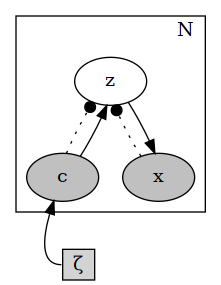
\includegraphics[width=0.4 \textwidth]{plots/cvae.gv.png}
\caption{Graphical model of the CVAE with a learned prior $p(\z | c)$.
as usual the solid arrows depict the inference model (encoder) and the dotted
ones the generative model (decoder)}
\label{fig:cvae}
%\end{framed}
\end{figure}

Figure~\ref{fig:cvaeumap} shows in the left a umap plot of the latent space for
the CVAE model which we described first, on the MNIST data set.
It uses the learned prior $p(\z|c)$ and
$\x$ and $c$ are conditionally independent given $\z$.
The middle image shows the reconstruction of the clusters centers (the means of
$p(\z | c)$). In this model the encoder completely separates the categories in
the latent representation, resulting in distinct blobs.
The right image is the CVAE described last, the one which "forgets" the
category, with fixed prior $p(\z | c) = p(\z) = \NN(\z;0,1)$.
In this model $\x$ is not conditionally independent from $c$, but instead it 
is directly dependent on both $\z$ and $c$ ($p(\x | \z, c)$).
The result is an encoding which mixes a lot of the categories in the latent
space but we can still notice some clustering.

\begin{figure}[h]
%\begin{framed}
\centering
\begin{subfigure}[b]{0.33\textwidth}
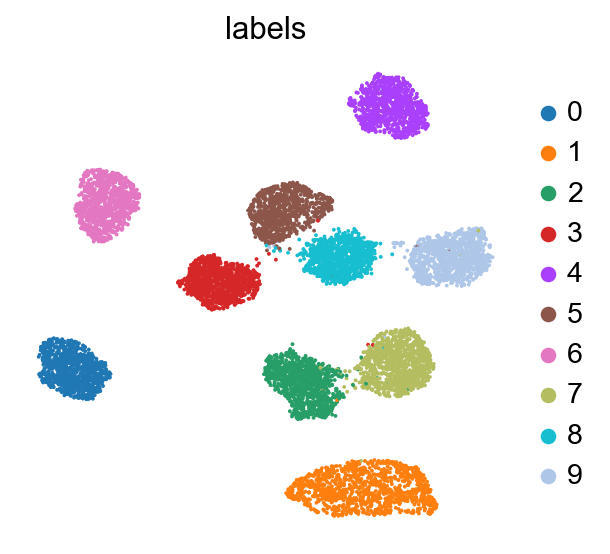
\includegraphics[width=\textwidth]{images/cvae2lp.umap.mnist.png}
\caption{learned prior}
\end{subfigure}
\begin{subfigure}[t]{0.33\textwidth}
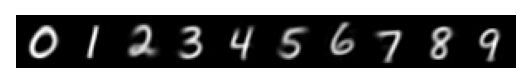
\includegraphics[width=\textwidth]{images/cvae2lp.clusterheads.mnist.png}
\caption{Reconstruction of the cluster centers}
\end{subfigure}
\begin{subfigure}[b]{0.33\textwidth}
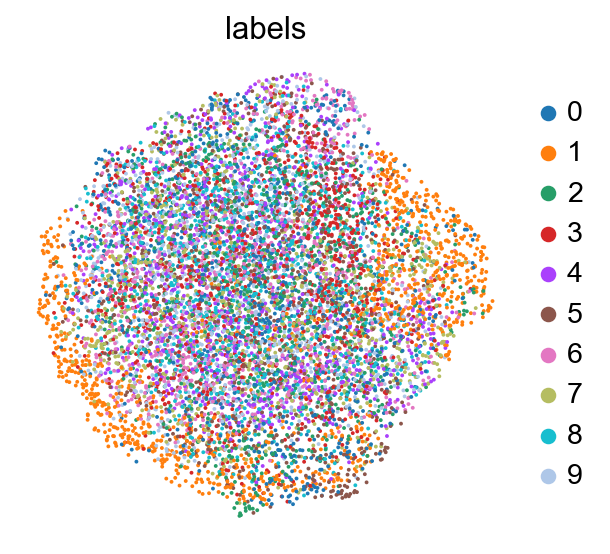
\includegraphics[width=\textwidth]{images/cvae1nolp.umap.mnist.png}
\caption{no learned prior}
\end{subfigure}
\caption{CVAE, different use cases}
\label{fig:cvaeumap}
%\end{framed}
\end{figure}

\chapter{Gaussian mixture model VAEs}
\section{Motivation}

Suppose that we have data of type $(\x,\y)$ which like in the CVAE case has numerical and 
categorical information, but unlike in the CVAE section we don't have access to
the categories $\y$, only to $\x$. 
We are looking for a model that can partition
$\X$ according to the true categories.
This is a task of unsupervised learning which is much harder then classifying
data with known targets $\Y$.

The original data has a complex distribution. Not only is it high dimensional,
but because the data belongs to distinct categories, it is natural to assume
that $\x$ comes from a mixture distribution.

We want to create some mixture distribution, where a latent categorical random
variable $\y$ functions as the component selector. We could try to directly
create the mixture $p(\x | \z, \y)$ in the $\x$ space, as the M2 model
in~\cite{kingma2014semi}.
The other option, following the Gaussian mixture model proposed by
Dilokthanakul et.al~\cite{dilokthanakul2016deep} and which base our model
is to create a mixture prior distribution $p(\z | \w, \y)$ on the lower
dimensional latent $\z$ space.

There are several advantages to doing this. For once we are interested in
dimensionality reduction and not just in unsupervised classification. If we
create a mixture distribution in the latent space $\z$ we can then further
analyse it (by clustering algorithms for example) and plot it, for example with
UMAP. A second reason is that it may be easier to create a mixture Gaussian on
the simpler, lower dimensional space $\z$ rather than on the high dimensional
$\x$ space where the data occupies a complex hyper-surface.

%We need to specify the generative model and the inference model as explained in
%section~\ref{VAE-specs}.
%We have just one type of observed random vector, $\x$ (the numerical data, for
%example corresponding to image if we deal with image dataset).
%
%We will certainly need a latent random vector $\y$ representing the categories 
%(in relaxes one-hot encoding). And we will need a random vector $\z$ to
%reconstruct $\x$ from.
%Instead we'll add another latent variable $\w$, and create a mixture
%distribution in $\z$, $p(\z | \w, \y)$. Then reconstruct $\x$ just from $\z$
%like in a vanilla VAE.

\begin{figure}[h]
%\begin{framed}
\centering
\begin{subfigure}[b]{0.4\textwidth}
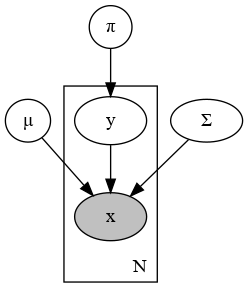
\includegraphics[width=\textwidth]{plots/mm.gv.png}
\caption{"vanilla" Gauss mixture model with fixed centroids.}
\label{fig:vanillamix}
\end{subfigure}
\begin{subfigure}[t]{0.4\textwidth}
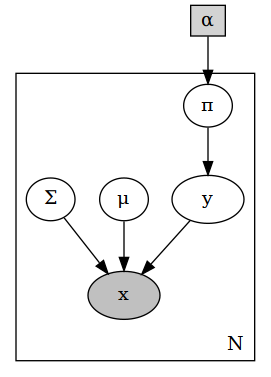
\includegraphics[width=\textwidth]{plots/mmp.gv.png}
\caption{a more complex mixture where the centroids are moved into the plate.}
\label{fig:platemix}
\end{subfigure}
\caption{}
\label{fig:mixturemodels}
%\end{framed}
\end{figure}

Figure~\ref{fig:vanillamix} describes the usual Gaussian mixture
model~\cite{bishop2006pattern}. The components'
centroids, $\bv{\mu} = (\bv{\mu}_1, \dots \bv{\mu}_k)$, its covariances,
$\bv{\Sigma}$, 
and the categorical selection
distribution $\pi$, are outside the plate.
It means we draw the centroids, variances, and the categorical distribution
once, and use them for all the samples inside the plate.
That constraints each category to be
distributed around some fixed center which is pretty restrictive and perhaps too
much so. By moving the random vectors inside the plate
(figure~\ref{fig:platemix}), we create a much more flexible distribution.

\begin{figure}[h]
%\begin{framed}
\centering
\begin{subfigure}[b]{0.4\textwidth}
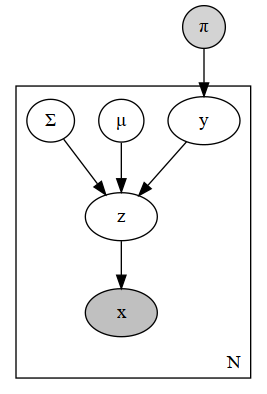
\includegraphics[width=\textwidth]{plots/mmpd.gv.png}
\caption{The generative model of GMMVAE~\cite{dilokthanakul2016deep}}
\label{fig:dilomix}
\end{subfigure}
\begin{subfigure}[b]{0.4\textwidth}
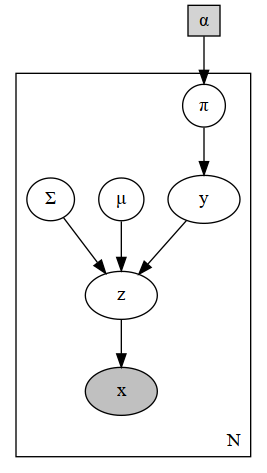
\includegraphics[width=\textwidth]{plots/mmpp.gv.png}
\caption{modified model}
\label{fig:mymix}
\end{subfigure}
\caption{
On the left we see the generative model used by
GMMVAE~\cite{dilokthanakul2016deep}, where $\pi$ is a fixed hyper parameter and resides
outside of the plate.
On the right: modification of the GMMVAE model, where $\pi$ moves inside the plate
and becomes a variable with a symmetric Dirichlet prior.}
\label{fig:mixturemodels2}
%\end{framed}
\end{figure}

Another issue with the original mixture model, if we try to base a VAE model on
it, is that it imposes a "bad categorical prior" on $\y$. We usually set $p(\y) \sim
\text{Cat}(\pi)$ and $\pi=\frac{1}{k}$ assuming the data is balanced. The
problem is that we want the inference model (the encoder) $q(\y | \x)$ to be a
good classifier so we don't want to impose it to be close to uniform. 
If we move
$\pi$ inside and give it a symmetric Dirichlet prior, we allow more
flexibility on $\pi$, so it can be be heavily biased towards one category, making it a good
predictor. $\alpha$ is a symmetric Dirichlet hyper-parameter and "tweaking" with
it has influence on the number of non-empty categories that the model finds
during training.

Figure~\ref{fig:dilomix} shows the generative model of the 
GMMVAE~\cite{dilokthanakul2016deep}, where the mixtures components ($\mu, \sigma$)
are inside the plate but the selection distribution $(\pi)$ is a fixed parameter
which is outside the of the plate.
The latent $\z$ space is a mixture distribution. As explained above, the $\y$-prior is
"bad" because it will be uniform categorical, while we want to use the inference
model $q(\y | \z)$ to predict the category.
In figure~\ref{fig:mymix} $\pi$ is moved inside the plate and becomes a variable. Its prior is a
symmetric Dirichlet with hyper-parameter $\alpha$.
We call our modification the \emph{DGMMVAE} model (D stands for the Dirichlet prior
obviously).

\section{The DGMMVAE model}

Our DGMMVAE model is based on figure~\ref{fig:mymix}.
In addition to the latent variables $\z$ (mixture), and $\y$ (categorical), there
$2$ more variables.
The third latent variabel $\w$ has standard normal prior.
With $\w$ the model generates the means and variances $\mu,
\sigma$ for the mixture's components, by a of neural network.
A fourth variable $\dd$ is the Dirichlet prior.
The full generative model factors as (figure~\ref{fig:dirgmm}):

\begin{equation}
\begin{aligned}
&p(\x, \y, \z, \w, \dd) &=\quad& 
p(\x | \z) p(\z | \w, \y) p(\y | \dd) p(\dd) p(\w) \\
&p(\w) &=\quad& \NN(\w | \bv{0},\bv{1}) \\
&p(\dd) &=\quad& \text{Dir}(\dd | \alpha) \\
&p(\y | \dd) &=\quad& \text{Cat}(\y | \dd) \\
&p(\z | \w, \y) &=\quad& \NN(\z | \mu(\w)_{\y}, \sigma(\w)_{\y})) \\
&p(\x | \z) &=\quad& \NN(\x | \mu(\z), \sigma(\z))
\label{eq:gmmfact}
\end{aligned}
\end{equation}

$\mu(\w), \sigma(\w), \mu(\z), \sigma(\z)$ are neural networks of the decoder.
$\mu(\w)$, ($\sigma(\w)$) is not just one mean (variance) but a set of $k$ (=number of categories)
means (variances), 
and we are selecting the component $\mu(\w)_{\y}, \sigma(\w)_{\y}$
indicated by $\y$, the categorical random
variable.

The generative process can be described as follows:
\begin{enumerate}
\item{} draw from the prior $\w \sim p(\w) = \NN(\w|\bv{0},\bv{1})$
\item{} draw a categorical distribution from the Dirichlet prior
$\dd \sim p(\dd) = \text{Dir}(\dd | \alpha)$
\item{} draw a category $\y \sim p(\y | \dd) = \text{Cat}(\y | \dd)$
\item{} generate the $k$ centroids and diagonal variances by the decoder's NN:
$\bv{\mu}(\w), \bv{\sigma}(\w)$.
\item draw from the mixture $\z \sim p(\z | \w,\y) = \NN(\z|\bv{\mu}(\w)_{\y},
\bv{\sigma}(\w)_{\y})$
\item{} generate the means $\bv{\mu}(\z)$ and diagonal variances
$\bv{\sigma}(\z)$ (or use fixed variance $1$) by the decoder NN.
\item{} draw observation $\x \sim p(\x | \z) = \NN(\x|\bv{\mu}(\z))$
\end{enumerate}

There are several ways to factor the inference model and it is not immediately
clear which one is better. Here is the factorization depicted in
figure~\ref{fig:dirgmm}:

\begin{equation}
\begin{aligned}
&q(\y, \z, \w, \dd | \x) &=& 
&q(\z | \x) q(\w | \x) q(\y | \z) q(\dd | \z) \\
&q(\z | \x) &=& &\NN(\z | \mu_z(\x), \sigma_z(\x)) \\
&q(\w | \x) &=& &\NN(\w | \mu_w(\x), \sigma_w(\x)) \\
&q(\y | \z) &=& &\text{Cat}(\y | f(\z)) \\
&q(\dd | \z) &=& &\text{Dir}(\dd | g(\z))
\label{eq:gmmqfact}
\end{aligned}
\end{equation}

And $f(\z),g(\z), \mu_w(\x), \sigma_w(\x), \mu_z(\x), \sigma_z(\x)$ are
the neural networks of the encoder.


\begin{figure}[h]
%\begin{framed}
\centering
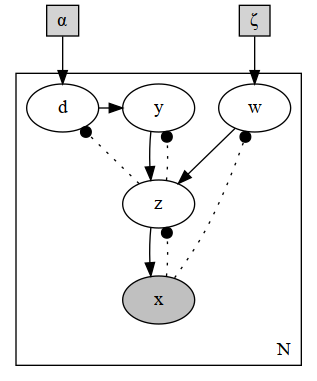
\includegraphics[width=0.5\textwidth]{plots/dirichlet_gmm.gv.png}
\caption{DGMMVAE: GMMVAE with Dirichlet prior}
\label{fig:dirgmm}
%\end{framed}
\end{figure}

\section{Computing the loss function of DGMMVAE model}

The loss function remains the -ELBO and we can break it into
different terms:

\begin{IEEEeqnarray}{lC}
\LL(p,q,\x) &= 
\int - \log \frac{p(\x,\y,\z,\w,\dd)}{q(\z,\y,\w,\dd | \x)} dq(\z,\y,\w,\dd |
\x) \\ 
&= \int - \log 
\frac{p(\x | \z) p(\z | \w, \y) p(\y | \dd) p(\w) p(\dd)}
{q(\z | \x) q(\w | \x) q(\y | \z) q(\dd | \z)} dq \\
&= \int - \log p(\x | \z) dq \\
\label{dgmmrecloss}
&+ \int \log \frac{q(\z | \x)}{p(\z | \w, \y)}dq \\
\label{dgmmzloss}
&+ \int \log \frac{q(\w | \x)}{p(\w)}dq \\
\label{dgmmwloss}
&+ \int \log \frac{q(\y | \z)}{p(\y | \dd)}dq \\
\label{dgmmyloss}
&+ \int \log \frac{q(\dd | \z)}{p(\dd)}dq
\label{dgmmdloss}
\end{IEEEeqnarray}

As we see there are five terms in the reconstruction loss function.
\ref{dgmmrecloss} is called the reconstruction error.
The rest of the terms get the repetitive, mundane names:
\ref{dgmmzloss} is called the $z$-error or $z$-kl-term,
\ref{dgmmwloss} is the $w$-error or $w$-kl-term,
\ref{dgmmyloss} is the $y$-error or $y$-kl-term, and
\ref{dgmmdloss} is called the $d$-error or $d$-kl-term.
%\subsection{Relation between AE and VAE}

To actually compute the loss function we will use Monte Carlo integration,
with one sample for each observation.
We will need to sample $\z$, $\w$ and $\dd$. For $\y$ we will not sample but
rather integrate over the categorical probabilities.


\begin{enumerate}
\item{sample} $\z \sim q(\z | \x)$ using the reparameterization trick
\item{sample} $\w \sim q(\w | \x)$ using the reparameterization trick
\item{sample} $\dd \sim q(\dd | \z)$ using the reparameterization trick
\item{Reconstruction error estimation}:
$$-\log p(\x | \z) = -\log \NN(\x | \mu(\z), \sigma(\z))$$
\item{$\z$-error}: calculate $KL(q(\z | \x) \| p(\z | \w, \y))$ analytically
using equation~\ref{eq:kldivnormal}
for every mixture component of $p(\z | \w, \y)$,
and then take the weighted average with respect
to $q(\y | \z)$:
$$\sum_{j=1}^k [ q(\y=j | \z) KL(q(\z | \x) \| p(\z | \w, \y=j))]$$.
\item{$\w$-error}: calculate $KL(q(\w | \x) \| p(\w))$ analytically 
the kl-divergence between two diagonal Gaussians (equation~\ref{eq:kldivnormal}).
\item{$\y$-error}:
calculate $KL(q(\y | \z) \| p(\y | \dd))$ analytically (kl-div of
two categorical distributions, ):
$$KL(q(\y | \z) \| p(\y | \dd)) = 
\sum_{j=1}^k [ q(\y=j | \z) \log \frac{q(\y=j | \z)}{p(\y = j | \dd)}]$$
\item{$\dd$-error}:
calculate $KL(q(\dd | \z) \| p(\dd))$ analytically
(kl-divergence of two Dirichlet distributions also has a closed formed
formula and it's builtin function in Pytorch).
\end{enumerate}

\section{The DGMMVAE model in the supervised case}

The DGMMVAE model can also be used for supervised training. While the
architecture of the neural network remains the same, the probabilistic
interpretation and consequently the calculation of the loss function is
different.

Figure~\ref{fig:dirgmm_sup} describes the generative and the inference model in
the supervised case.
Since in this case $\y$ is observed, we regard $\z$ in the generative model
as only dependent on $\w$. Internally we keep the same architecture but during
supervised training we always select just the given $\y$ component and so we
can stop regarding $\z$ as depending on $\y$.
$p(\z | \w, \y) = p(\z | \w) = \NN(\z | \mu(\w)_y, \sigma(\w)_y)$.
In the figure we show the dashed arrow from $\y$ to $\w$ but if it were a real
dependency we would get an "illegal" cycle in the $p$-graph. However the $\y$
which we used to select the $\mu(\w), \sigma(\w)$ mixture components are not
drawn from $p(\y | \z)$, rather we use the observation $\y$ (=the category
label) itself which is
given to us in the supervised case. Thus there is no actual cycle in the
dependency graph but the effect of $\y$ remains in the implementation of the
network architecture. 

Moreover in the supervised case the random variable $\y$ becomes dependent on both $\dd$ and $\z$.
We make an assumption that $\y | \dd$ and $\y | \z$ are independent, so
$p(\y | \dd, \z) = p(\y | \dd)p(\y | \z)$, thus enabling us to retain the same 
network architecture. $p(\y | \dd)$ is determined by
the same decoder component as in the unsupervised case but $p(\y | \z)$ equals 
$q(\y | \z)$ of the encoder in the unsupervised case. So while again we keep the same
architecture we will compute the loss function differently.
As for the inference model it becomes other than losing the $q(\y | \z)$
component the rest remains the same.
The full factorization in the supervised case becomes:

\begin{equation}
\begin{aligned}
&p(\x, \y, \z, \w, \dd) &=& 
&p(\x | \z) p(\y | \dd) p(\y | \z) p(\z | \w) p(\dd) p(\w) \\
&q(\z, \w, \dd | \x, \y) &=& 
&q(\z | \x) q(\w | \x) q(\dd | \z) \\
&p(\x | \z) &=& & \NN(\x | \mu(\z), \sigma(\z)) \\
&p(\y | \z) &=& &\text{Cat}(\y | f(\z)) \\
&p(\y | \dd) &=& & \text{Cat}(\y | \dd) \\
&p(\w) &=& & \NN(\w | \bv{0},\bv{1}) \\
&p(\dd) &=& & \text{Dir}(\dd | \alpha) \\
&p(\z | \w) &=& & \NN(\z | \mu(\w)_{\y}, \sigma(\w)_{\y})) \\
&q(\z | \x) &=& &\NN(\z | \mu_z(\x), \sigma_z(\x)) \\
&q(\w | \x) &=& &\NN(\w | \mu_w(\x), \sigma_w(\x)) \\
&q(\dd | \z) &=& &\text{Dir}(\dd | g(\z))
\label{eq:gmmfact_supervised}
\end{aligned}
\end{equation}

\begin{figure}[h]
%\begin{framed}
\centering
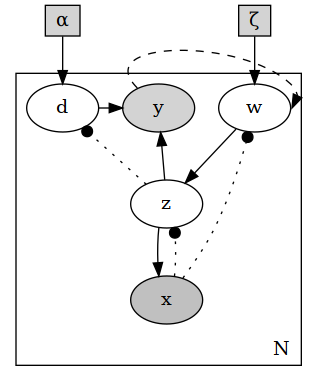
\includegraphics[width=0.5\textwidth]{plots/dirichlet_gmm_supervised.gv.png}
\caption{DGMMVAE: the supervised case, where $\y$ is an observed variable.
}
\label{fig:dirgmm_sup}
%\end{framed}
\end{figure}
%\subsection{Conditional VAE}

The loss function in the supervised case is:

\begin{IEEEeqnarray}{lC}
\LL(p,q,\x) &= 
\int - \log \frac{p(\x,\y,\z,\w,\dd)}{q(\z,\w,\dd | \x, \y)} dq(\z,\y,\w,\dd |
\x) \\ 
&= \int - \log 
\frac{p(\x | \z) p(\z | \w) p(\y | \dd) p(\y | \z) p(\w) p(\dd)}
{q(\z | \x) q(\w | \x) q(\dd | \z)} dq \\
&= \int - \log p(\x | \z) dq \\
\label{dgmmrecloss}
&+ \int \log \frac{q(\z | \x)}{p(\z | \w)}dq \\
\label{dgmmzloss}
&+ \int \log \frac{q(\w | \x)}{p(\w)}dq \\
\label{dgmmwloss}
&+ \int \log p(\y | \z)dq \\
&+ \int \log p(\y | \dd)dq \\
\label{dgmmyloss}
&+ \int \log \frac{q(\dd | \z)}{p(\dd)}dq
\label{dgmmdloss_supervised}
\end{IEEEeqnarray}

The reconstruction error, the $w$-error and the $d$-error are calculated exactly
like in the unsupervised loss.
The $z$-term is also calculated in exactly the same procedure as in unsupervised
case except that we only need to take the component indicated by the obseved
$\y$ in the weighted sum.
The two $y$-terms are the log probability of the observed category given the
sampled $\z$ and $\dd$.

\section{Combining GMMVAE with another clustering method}

Because GMMVAE performs particularly well in (semi)supervised 
it can learn a given cluster/class assignment of a dataset by.
But when might it be useful to train GMMVAE if we already have a different
clustering algorithm or any other unsupervised classifier that works well?
Suppose that we have a "nice" training set where a given clustering algorithm
performs well on.
We can supervised train GMMVAE on the nice dataset using the cluster assignment
as labels. At this point the model should learn to represent the data clusters
nearly perfect.
It is often the case that the GMMVAE trained in this manner will out-perform 
a "naive" GMMVAE which was unsupervised trained.

We can than run unsupervised training on the dataset, if we are
lucky the accuracy might improve. So that's one use case but a minor one.

The more important usage is that we can now classify with GMMVAE other datasets
of the same kind.
We should compare the performance of the trained model on the testing set with
the performance of the clustering algorithm \emph{on the testing set} which per
assumption was not that good. If we are lucky the GMMVAE might outperform the
clustering algorithm on the not--so--nice testing data.

We tested a combination of GMMVAE with Louvain~\cite{que2015scalable} clustering
on several datasets (results shown in subsequent chapters).


\section{The conditional mixture model, cDGMMVAE}
%\section{Motivation}

We have seen two types of models that deal with data that is both numerical and
categorical, namely the conditional VAE (CVAE), and the GMMVAE.
The cDGMMVAE is a combination of both, a conditional DGMMVAE. 
It is technically very easy to implement a conditional version from a 
given VAE model. Basically it just requires 
concatenating the condition $c$ to whatever variable we want to condition.
But why do we need it?

Suppose that we have again numerical/categorical type of data $(\x, \y)$ which 
comes in two or more types of "flavors" $c$, so the full data type 
is $(\x, \y, c)$. For example $\x$ can be an image of on of $k$ 
different faces, 
$\y$ is the identity of the person, $c$ is an indicator of whether the person
smiles or not. 
Also suppose that $\y$ might not be provided at all or just for
a subset of the data but $c$ is always provided for us.

The data we actually use for this model is scRNAseq data that comes from two types 
of conditions (control and stimulated), 
which are the conditions before and after exposure to some pathogen or some chemical.
$\x$ is normalized gene expression levels, $\y$ is the cell type 
we want to infer but may not know the ground truth, and $c$ indicates from which
group the measurement was taken (control/stimulate) and this information is
visible to use because we know for each sample from which group it was
taken.


\begin{figure}[h]
%\begin{framed}
\centering
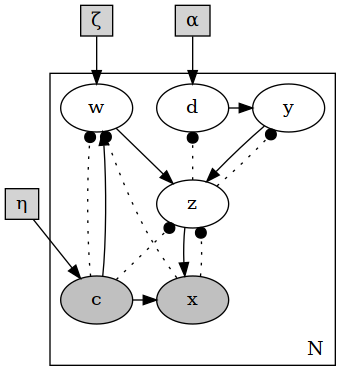
\includegraphics[width=0.5\textwidth]{plots/dirichlet_gmm_cvae.gv.png}
\caption{cDGMMVAE, unsupervised case}
\label{fig:dirgmmcvae}
%\end{framed}
\end{figure}

\begin{figure}[h]
%\begin{framed}
\centering
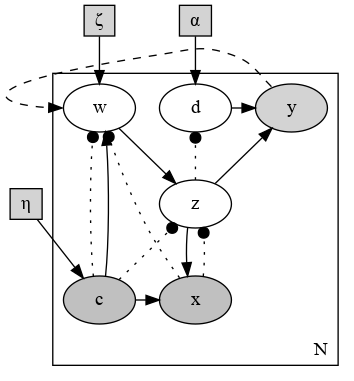
\includegraphics[width=0.5\textwidth]{plots/dirichlet_gmm_cvae_supervised.gv.png}
\caption{cDGMMVAE, supervised case}
\label{fig:dirgmmcvae_super}
%\end{framed}
\end{figure}

The factorization in the unsupervised case is:

\begin{equation}
\begin{aligned}
&p(\x, \y, \z, \w, \dd, c) &=& 
&p(\x | \z, c) p(\z | \w, \y) p(\y | \dd) p(\dd) p(\w | c) \\
&q(\z, \w, \dd | \x, \y, c) &=& 
&q(\z | \x, c) q(\w | \x, c) q(\y | \z) q(\dd | \z)
\label{eq:cgmmfact_unsupervised}
\end{aligned}
\end{equation}

And in the supervised case:

\begin{equation}
\begin{aligned}
&p(\x, \y, \z, \w, \dd, c) &=& 
&p(\x | \z, c) p(\y | \dd) p(\y | \z) p(\z | \w) p(\dd) p(\w | c) \\
&q(\z, \w, \dd | \x, \y) &=& 
&q(\z | \x, c) q(\w | \x, c) q(\dd | \z)
\label{eq:cgmmfact_supervised}
\end{aligned}
\end{equation}

In this model we want to keep the dependency of $\x$ on $c$, hence
$p(\x | \z, c)$. This allows us to "flip" condition of the reconstruction,
which we can interpret as converting for example control cells to stimulated
cells, as we'll see in a later chapter.


\chapter{Experiments and results MNIST}
%\section{Tests with MNIST and FMNIST}

The first dataset we tested the model on was MNIST~\cite{mnist} which is 
easy to machine learn yet it is also the most tested and compared dataset.
This is a collection of $28 \times 28$ pixel gray--scale images of hand written 
digits. The images are labeled with the ground truth so it is an $(\X,\Y)$ kind
of data, with $\X$ being numerical and $\Y$ categorical.

MNIST images are close to being binary black and wight (either close to $0$ or
close to $1$), so it is better to model them with Bernoulli distribution than
with Gaussian, with the intensity of each pixel is regarded as a Bernoulli
probability.
Unless otherwise stated, for MNIST we set $p(\x | \z)$ to be Bernoulli
distribution.

\section{semi-supervised learning}

In the first test we partition the training set into labeled
($5\%$ of the total) and unlabeled subset (the other $95\%$).
As we have some labeled images, we set the number--of--categories hyperparameter
on $10$ and the goal here is to be able to predict the true categorical
partitioning of the testing set.

There are several qualitative aspects that we are particularly interested in
this experiment:

\begin{itemize}
\item{} The overall prediction accuracy of the model
\item{} Comparing the models predicted clusters to Louvain clusters
\subitem{} in the PCA space
\subitem{} in the latent space
\end{itemize}


\begin{figure}[h]
%\begin{framed}
\centering
\begin{subfigure}[b]{0.95\textwidth}
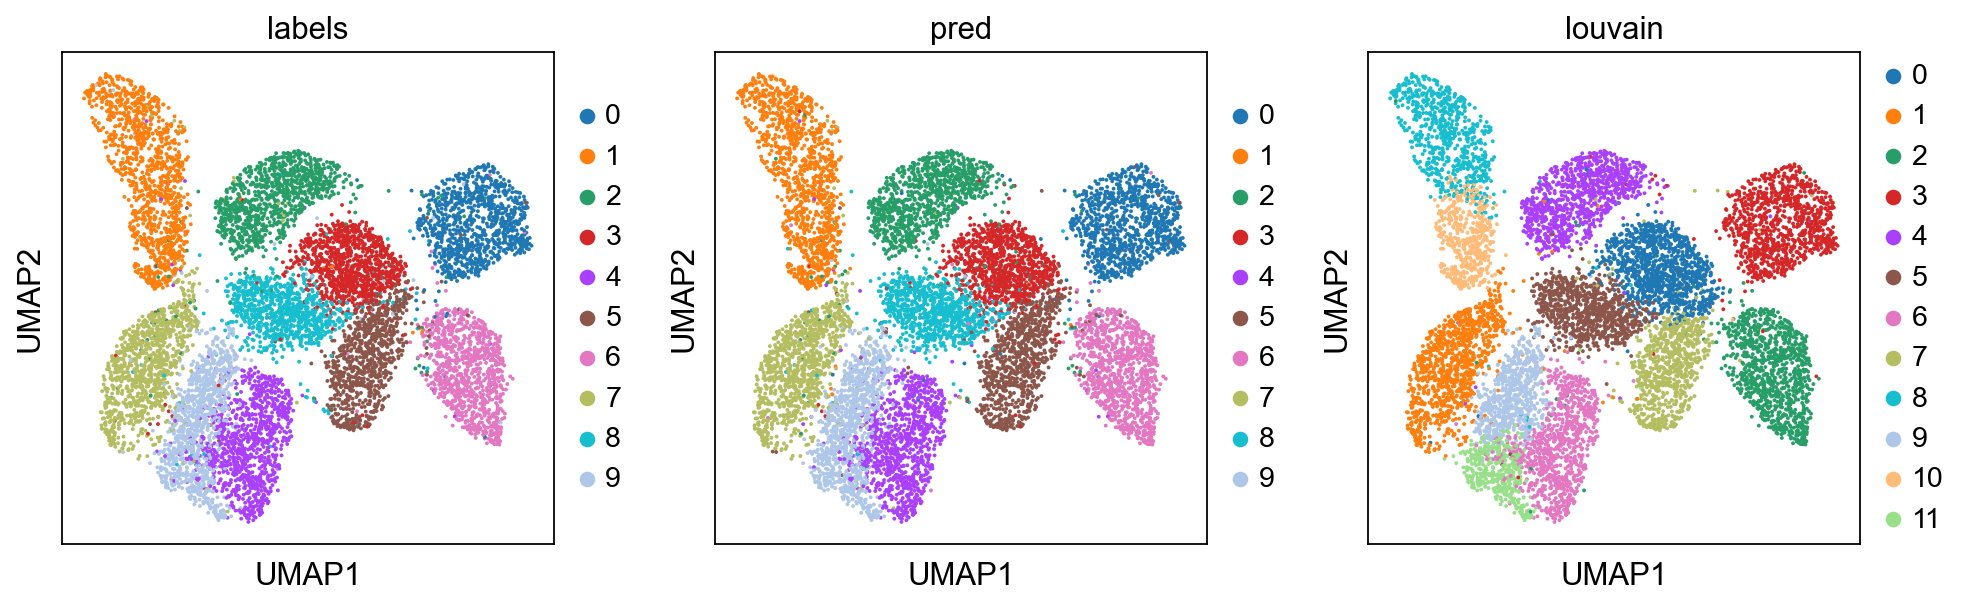
\includegraphics[width=\textwidth]{images/gmmvae_mnist_ss_pca_umap.png}
\caption{UMAP of the PCA space}
\label{fig:mnist_ss_pca}
\end{subfigure}
\begin{subfigure}[b]{0.95\textwidth}
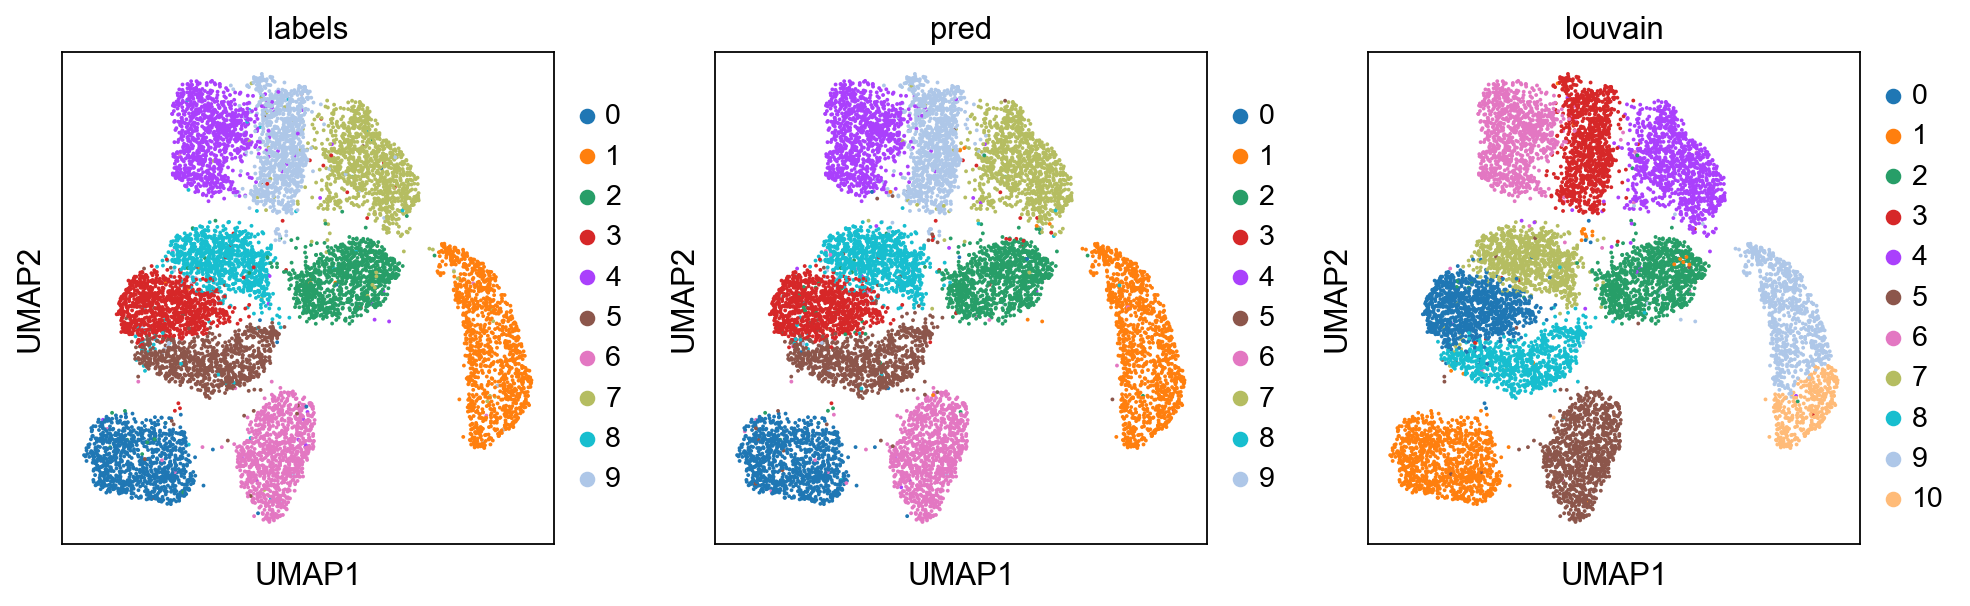
\includegraphics[width=\textwidth]{images/gmmvae_mnist_ss_latent_umap.png}
\caption{UMAP of the latent space}
\label{fig:mnist_ss_latent}
\end{subfigure}
\caption{Comparison of the predictive quality of the model vs. Louvain
clustering on the PCA space (top) and on the latent space (bottom).}
\label{fig:mnist_ss_umaps}
%\end{framed}
\end{figure}

The overall accuracy of the model is $0.955$ and as
the figures~\ref{fig:mnist_ss_umaps} the prediction basically identifies the
real classes.
When performed on the PCA space, Louvain clustering with default settings identifies $12$ clusters
. The "$0$" and "$9$" classes each are split
between two Louvain clusters. The Louvain clusters themselves appear to be
homogeneous (each cluster contain practically only samples from one ground-truth
class).

It is interesting to compare the PCA results to the same procedure done on the
latent space.
The umap appears a little bit better (the ground truth classes have more
separation from each other).
This time there are $11$ louvain clusters and only the "9"
category is split between two louvain clusters.
This is despite the latent $z$ space being only $16$-dimensional, while the PCA
is done on the $50$ most significant components.

\begin{figure}[h]
%\begin{framed}
\centering
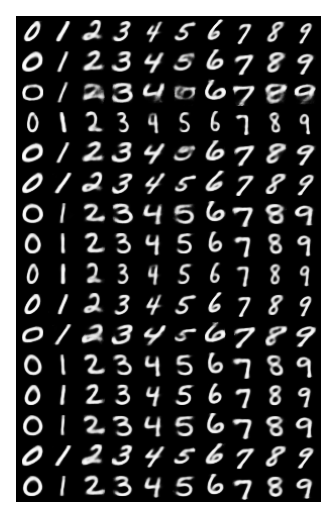
\includegraphics[width=0.3\textwidth]{images/gmmvae_mnist_ss_samples.png}
\caption{Images generated by random sampling from the latent mixture
distribution. As we can see it fits perfectly with the right ground truth
classes.}
\label{fig:mnist_ss_samples}
%\end{framed}
\end{figure}

Figure~\ref{fig:mnist_ss_samples} shows the decoder's reconstruction of random
samples from the mixture distribution which was imposed on the latent space.
As we can see each component generates exactly one of the digit classes.
Sampling from the latent mixture distribution ($z$-space) is done as follows:
Firs we take random samples from the $w$-space, on which we imposed a standard
normal diagonal distribution. Each sample corresponds to one row in the image.
Then each $w$-sample is projected by the decoder into $10$ (number of defined
classes) mixture component. Each of these component if then further projected by
the decoder network into the sample space ($x$). 

\section{Unsupervised learning}
\subsection{10 Clusters (exact clustering)}
Getting the model to learn exactly the $10$ ground truth classes is a daunting
task. It requires a lot of tuning and micromanaging of the training procedure.
In my experiments, the model first needs to be trained with standard learning
rate ($1e-3$) to the point where it can adequately reconstruct digits and uses
all $10$ classes. Then the learning rate should be reduced to the range $5e-2$
--- $5e-3$. This makes reconstruction less exact and allows the model to "jump"
class predictions during training. If the learning rate is too big
eventually the model might completely drift away and become inaccurate and
unstable and if it is not sufficiently large the model remains stuck 
on a suboptimal classification. 
After this course training finds the correct classes, it needs to be further
trained to improve accuracy and reconstruction with decreasing learning rates.

In my experiments, an accuracy of about $0.9$---$0.95$ can be achieved
however due the micromanagement involved it is hard to make the training fully
automated. Moreover it may be completely unrealistic to expect the model
to perform that well in unsupervised exact clustering tasks with harder
datasets. 

\begin{figure}[h]
%\begin{framed}
\centering
\begin{subfigure}[b]{1.01\textwidth}
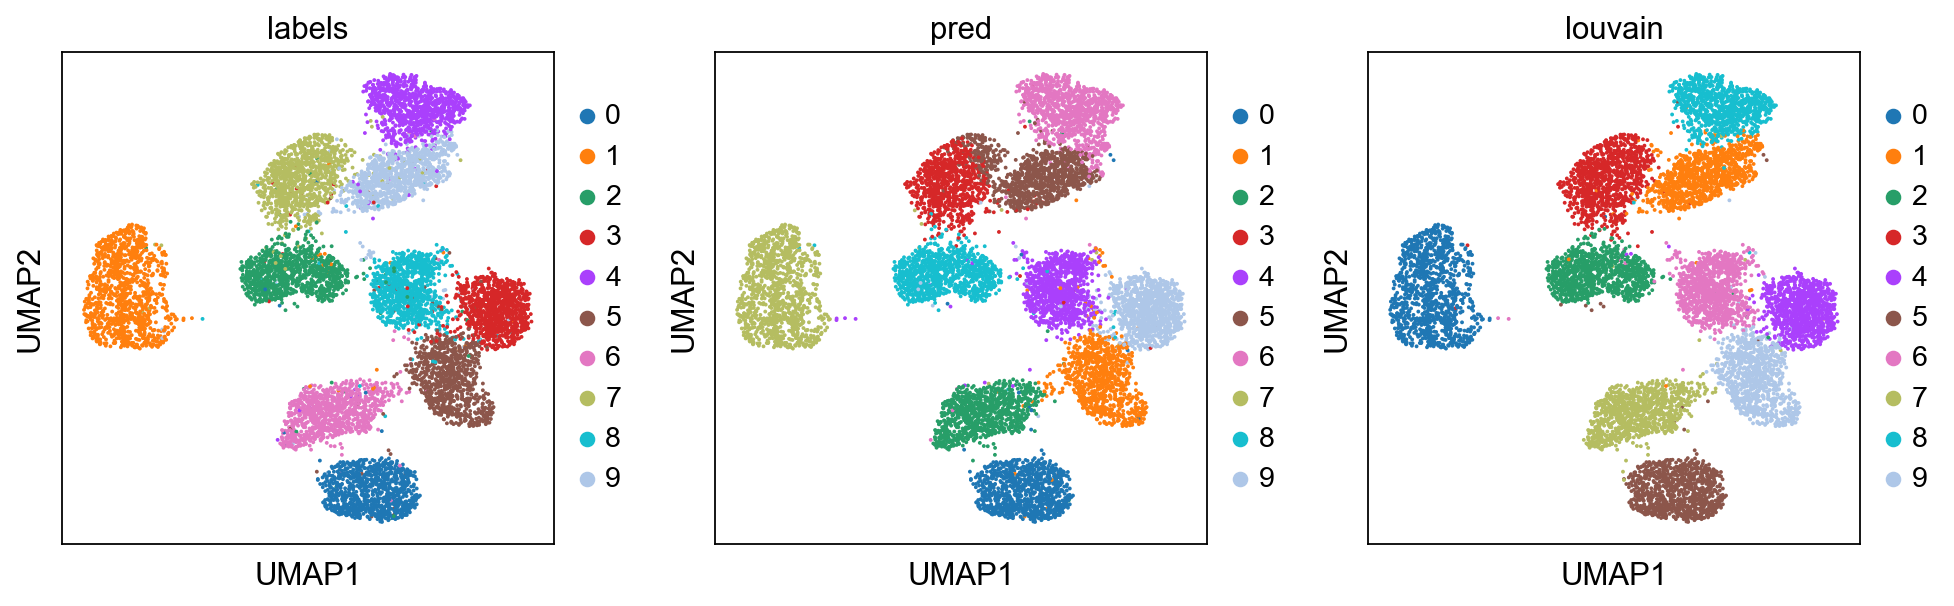
\includegraphics[width=\textwidth]{images/gmmvae_mnist_us_latent_umap.png}
\caption{UMAP of the latent space}
\label{fig:mnist_us_latent}
\end{subfigure}
\begin{subfigure}[b]{0.3\textwidth}
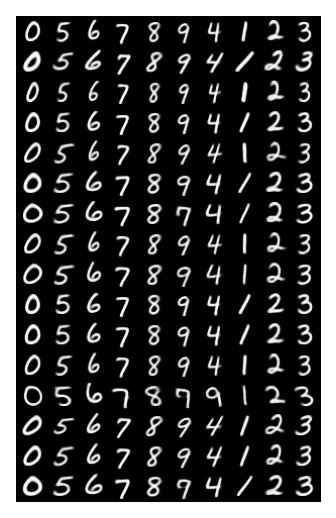
\includegraphics[width=\textwidth]{images/gmmvae_mnist_us_samples2.png}
\caption{Randomly generated samples}
\label{fig:mnist_us_samples}
\end{subfigure}
\caption{GMMVAE: unsupervised learning of MNIST. This particular model
achieved 0.93 accyracy which probably could be a little bit further
improved with fine-tune training. The Louvain clustering of the latent space is even better
than the prediction.}
\label{fig:mnist_us_10}
%\end{framed}
\end{figure}

Figures~\ref{fig:mnist_us_10} shows the results of unsupervised, exact clustering
of MNIST by the GMMVAE model with 8 dimensional latent $z$-space and
$w$-space.
As both the umap and the generated samples show, there is still a little bit
inaccuracies left, mainly with "7","4", and "9" digits.
Despite this, the actual latent space is very nicely clustered and louvain
clustering over this space retrieves the true classification of the the data
set, even to higher accuracy than the model prediction.
Note that in unsupervised learning the predicted classes are naturally untagged
with the ground truth class tag, the point is that it should find essentially
the true partitioning of the data. The tag assignment can be done later. for
example each predicted cluster is tagged with the class with which it has the
most overlap.

\subsection{With overclustering}
Overclustering means defining a mixture distribution with more components then
ground truth classes. This helps the model to create homogenous classes,
where each component is nearly a subset of a single class.
Moreover In the case of MNIST each digit has actually 2 or more basic appearance (e.g. 
strait vs. italic version, closed vs. open top "4" figure etc.). One can argue
that there are more "natural" classes in this dataset than the 10 digits.
We ran unsupervised training of a GMMVAE model with $20$ components.

\begin{figure}[h]
\centering
\begin{subfigure}[b]{1.01\textwidth}
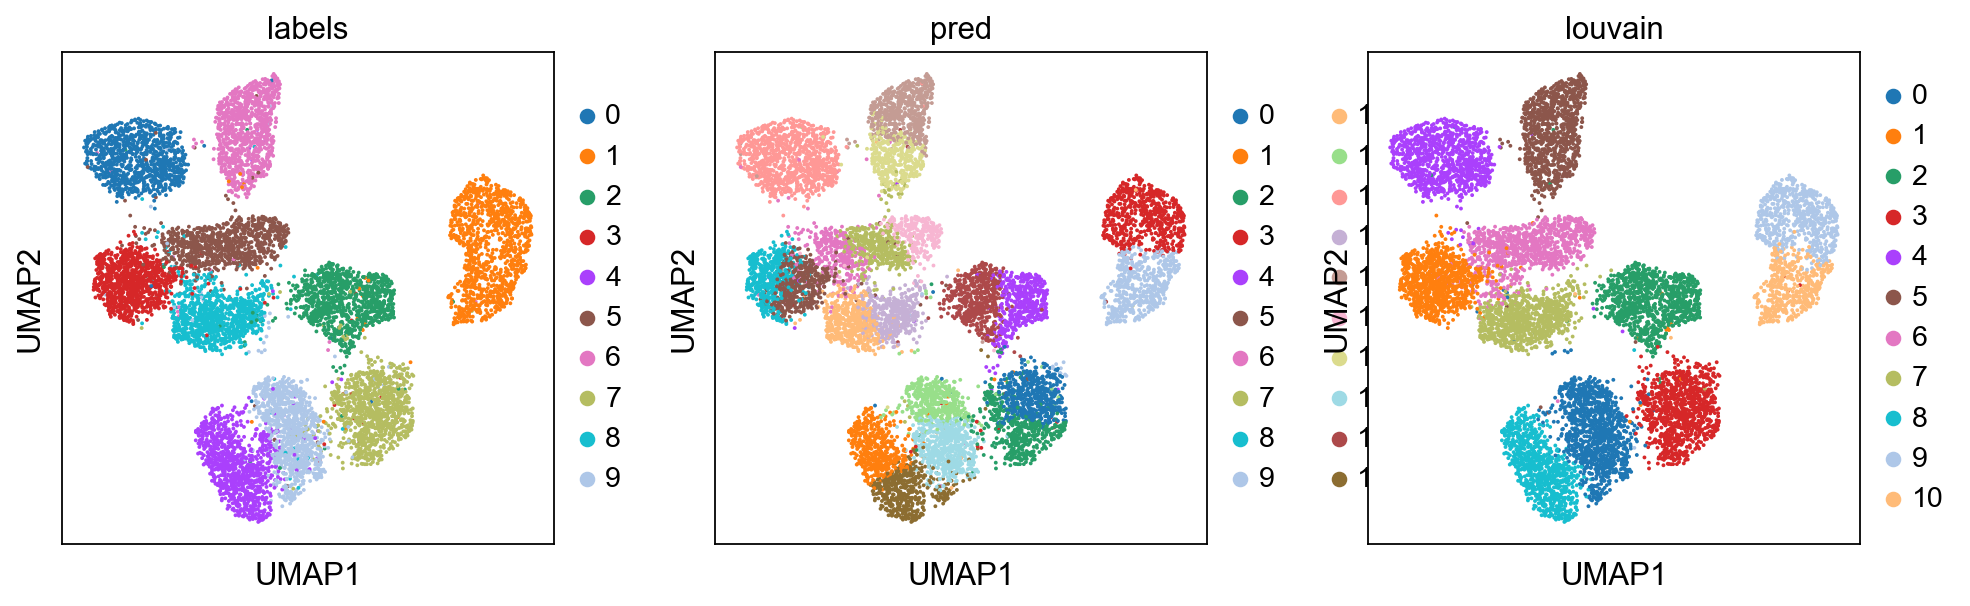
\includegraphics[width=\textwidth]{images/gmmvae_mnist_us_20c_umap4.png}
\caption{UMAP (20 components, MNIST)}
\label{fig:mnist_us_20c_latent}
\end{subfigure}
\begin{subfigure}[b]{0.5\textwidth}
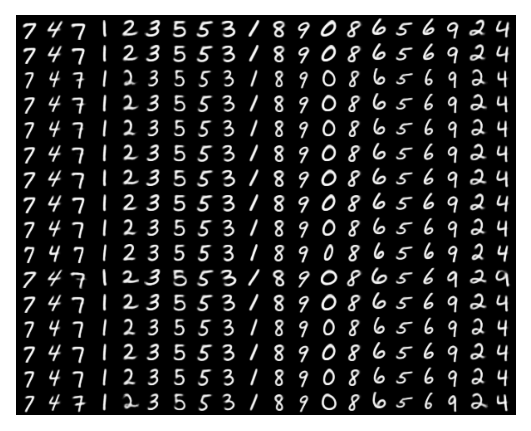
\includegraphics[width=\textwidth]{images/gmmvae_mnist_us_20c_samples4.png}
\caption{20 components: generated digits}
\label{fig:mnist_us_20c_samples}
\end{subfigure}
\caption{GMMVAE with 20 components, unsupervised learning of MNIST.}
\label{fig:mnist_us_20}
\end{figure}

Figures~\ref{fig:mnist_us_20} show the results of the 20--component GMMVAE
model. "0" constitutes its own cluster, while "5" is split between 3 clusters.
The rest of the classes are each split between two clusters. Each cluster has
its own digit-style (e.g. a strait "7" in one cluster, and more cursive version
in the other cluster). Unfortunately there is some misclassifications between
"4" and "9". Overall accuracy is about $0.946$, probably with some room for
improvement with additional training rounds. Louvain clustering of the latent
space is able to almost perfectly capture the true classes, with the "1" class
split between two Louvain clusters and the other classes correspond each to a
single Louvain cluster.

Training an overclustering model provides much more consistent results without
training micromanagement. It is probably advisable to set up a model with more
mixture components than the ground truth classes when trying unsupervised
classification of more complex datasets.

\section{Combination with Louvain clustering}

Louvain clustering achieves on its own an accuracy of 0.967 on the
\emph{training set} which is larger (60k images) and 0.925 on the smaller (10k) 
testing set.

We performed supervised training of GMMVAE model using Louvain clusters as the
labels.
After this step, the model was 0.966 accurate \emph{on the testing set}.
After further unsupervised training of the model the accuracy marginally
improved to 0.968.

MNIST is an easy data set but still the improvement over Louvain from 0.92 to 0.968 is
noticeable. There was also an improvement over the unsupervised model and it
basically solved the misclassification issue between 9,7 and 4 which is
the main problem we observes with unsupervised learning as we see in
figure~\ref{fig:mnist_us_louvain}.

\begin{figure}[h]
\centering
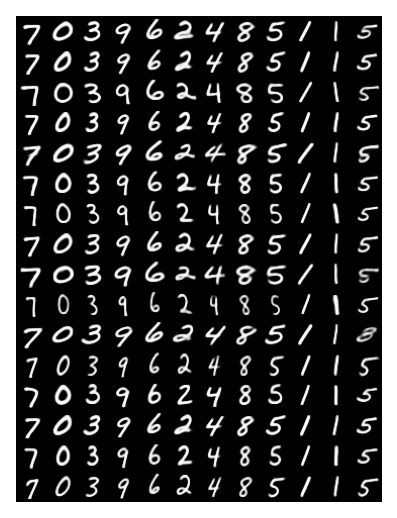
\includegraphics[width=0.4\textwidth]{images/gmmvae_mnist_us_louvain_samples1.png}
\label{fig:mnist_us_louvain_samples}
\caption{GMMVAE with 12 components guided by Louvain clustering: randomly generated digits}
\label{fig:mnist_us_louvain}
\end{figure}



\chapter{Experiments and results fashion-MNIST}
Fashion-MNIST (FMNIST)~\cite{fmnist} is a drop-in replacement for MNIST which
is a lot more challenging to machine--learn. Instead of digits we are dealing
here with greyscale images of clothing and accessory items of 10
classes:~
\emph{
T-shirt, trouser, pullover, dress, coat, sandal, shirt, sneaker, bag, boot.
}
Although each image is tagged with a single category, it is not always obvious
even for a human observer whether a certain image is actually a coat or a shirt,
for example. There might be a little bit of this type of unclaritty in MNIST
too, but it is much more pronounced in the fashion-MNIST dataset.

\section{Unsupervised learning}

GMMVAE achieved an overall $0.75$ accuracy after \emph{a lot} of training epochs.
It is easier to achieve about $0.67$ accuracy after a quick training (about 10
epochs).
Choice of hyperparameters also have significant effect. For example choosing 
a high dimensional latent space or deepening the networks tend to make the model
perform to not use all the components of the mixture.

\begin{figure}[h]
\centering
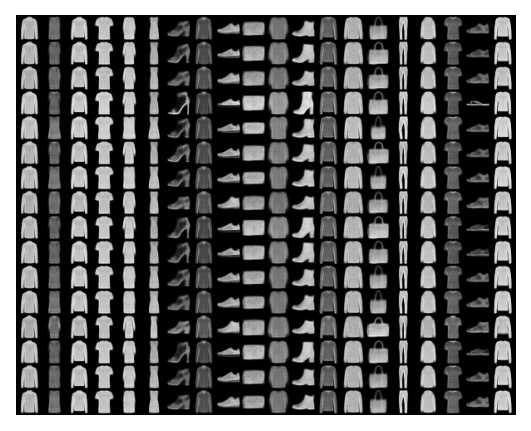
\includegraphics[width=0.6\textwidth]{images/gmmvae_fmnist_us_20c_samples0.png}
\caption{20 components: generated digits}
\label{fig:fmnist_us_20c_samples}
\end{figure}

\begin{figure}[h]
\centering
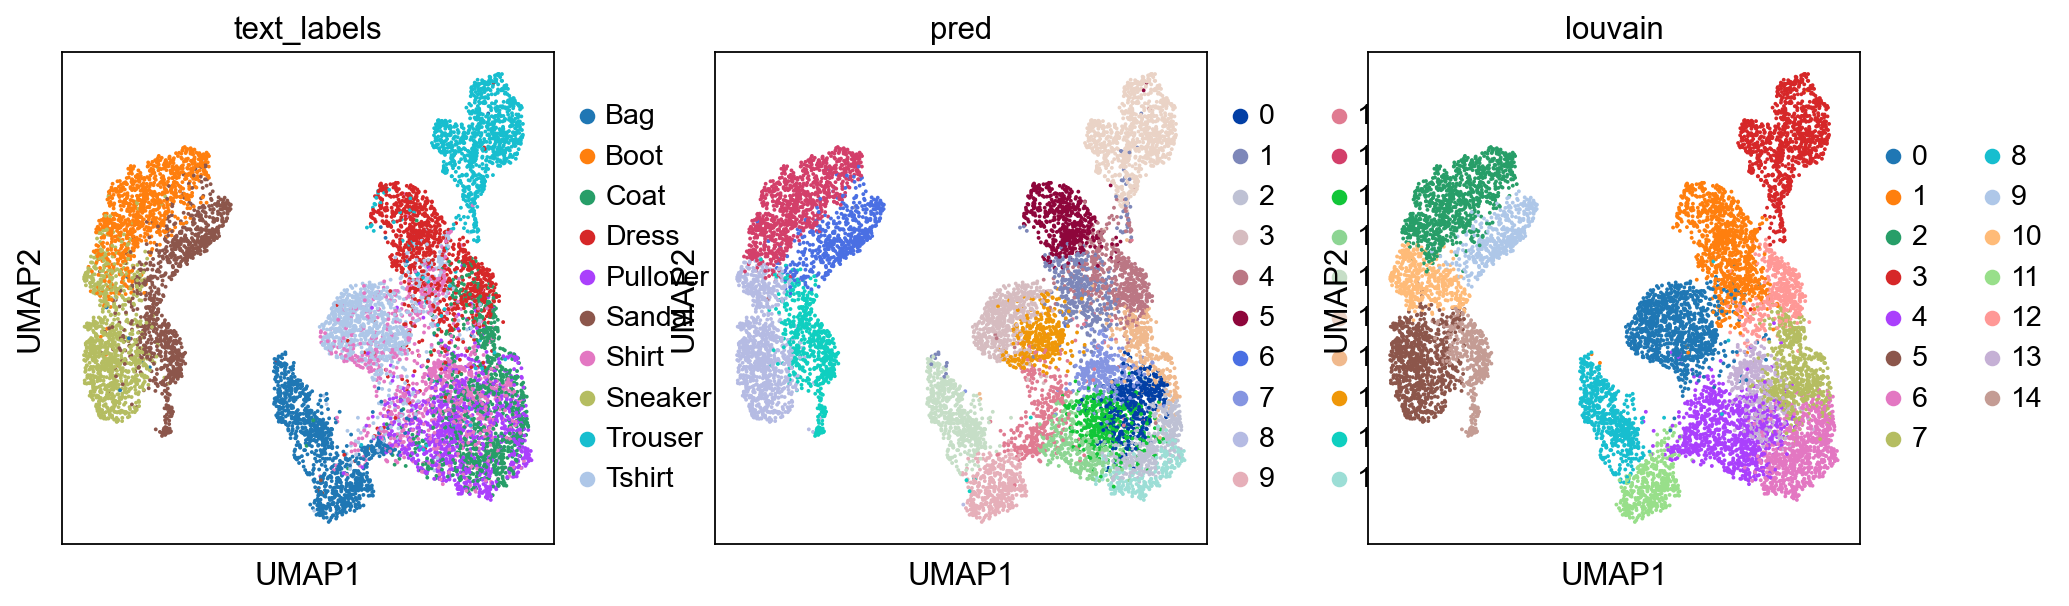
\includegraphics[width=0.9\textwidth]{images/gmmvae_fmnist_us_20c_umap0.png}
\caption{UMAP (20 components, MNIST)}
\label{fig:fmnist_us_20c_latent}
\end{figure}

Judging from the randomly generated images in
figure~\ref{fig:fmnist_us_20c_samples}, the model learns to 
generate what looks like a distinct classes in each of the mixture components.
However as far as prediction accuracy, there is a major confusion between
"shirt", "coat", and "pullover" classes, which is apparent from the UMAP in 
figure~\ref{fig:fmnist_us_20c_latent}.

\section{Semisupervised learning}

Our GMMVAE model achieved accuracy of $0.85$ on semisupervised learning with
$0.1$ --- $0.9$ split between known and hidden labels. 
Considering that this accuracy was semisupervised and that the network 
layer architecture we used was just fully connected with 2 hidden layers 
we think this accuracy is not bad.

\begin{figure}[h]
\centering
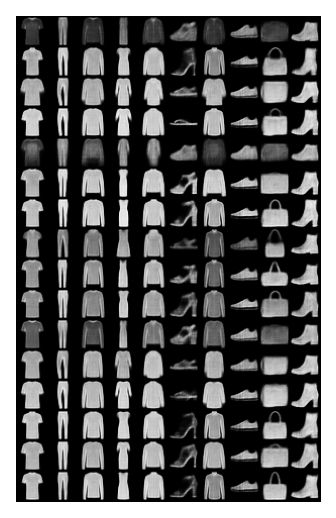
\includegraphics[width=0.5\textwidth]{images/gmmvae_fmnist_ss_samples.png}
\caption{FMNIST, semisupervised. Randomly generated samples.}
\label{fig:fmnist_ss_samples}
\end{figure}

Figure~\ref{fig:fmnist_ss_samples} shows randomly generated samples 
by the model. The $10$ components match the ground truth classes
fairly well.

\begin{figure}[h]
\centering
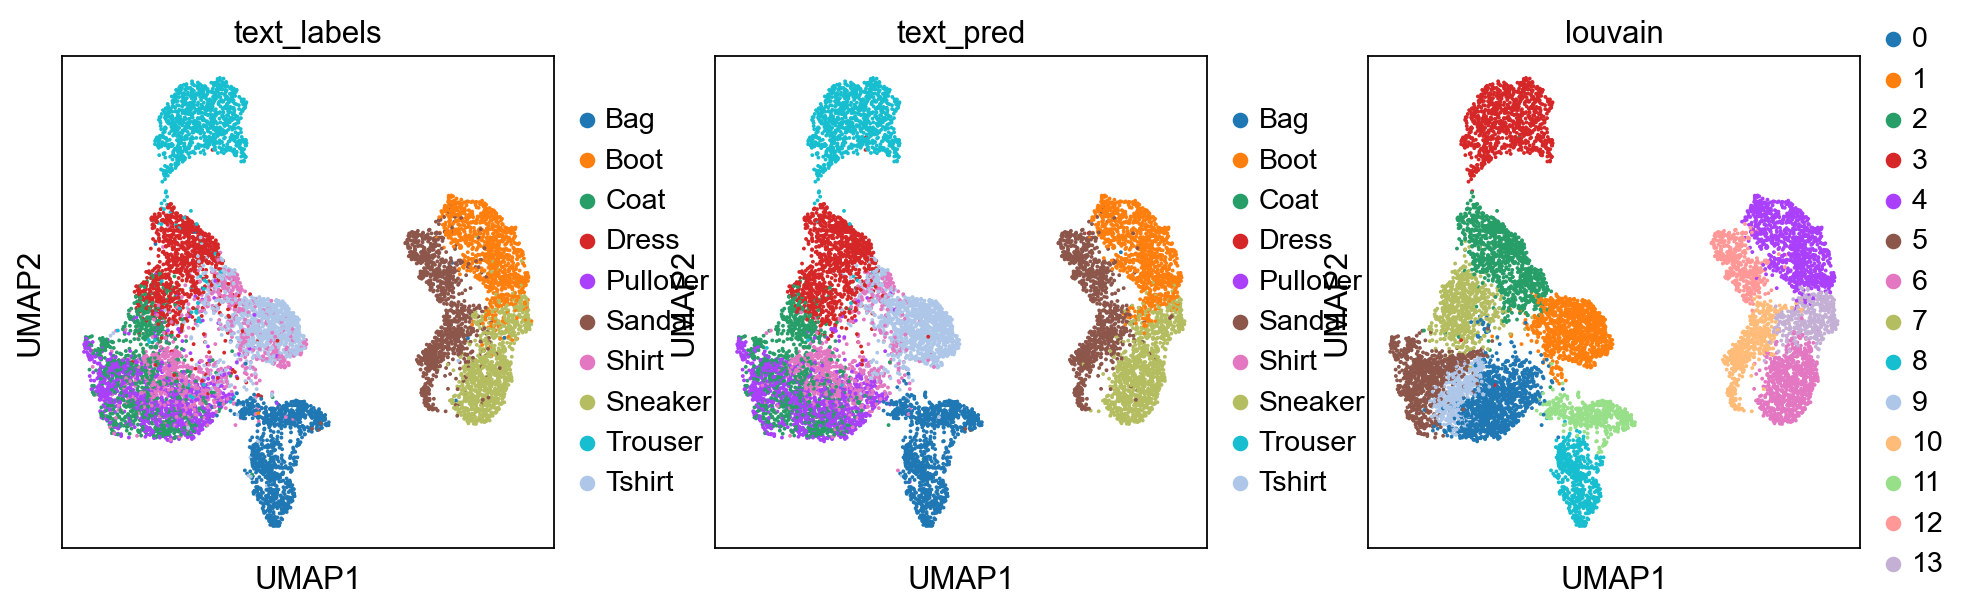
\includegraphics[width=1.1\textwidth]{images/gmmvae_fmnist_ss_latent_umap.png}
\caption{FMNIST, semisupervised. UMAP}
\label{fig:fmnist_ss_latent}
\end{figure}

Figure~\ref{fig:fmnist_ss_latent} shows UMAP of the laten space.
The top-wear (shirt, coat, pullover, T-shirt) are still pretty mixed and that's
where most of the misclassifications occur.

%\begin{figure}[h]
%\centering
%\begin{subfigure}[b]{1.01\textwidth}
%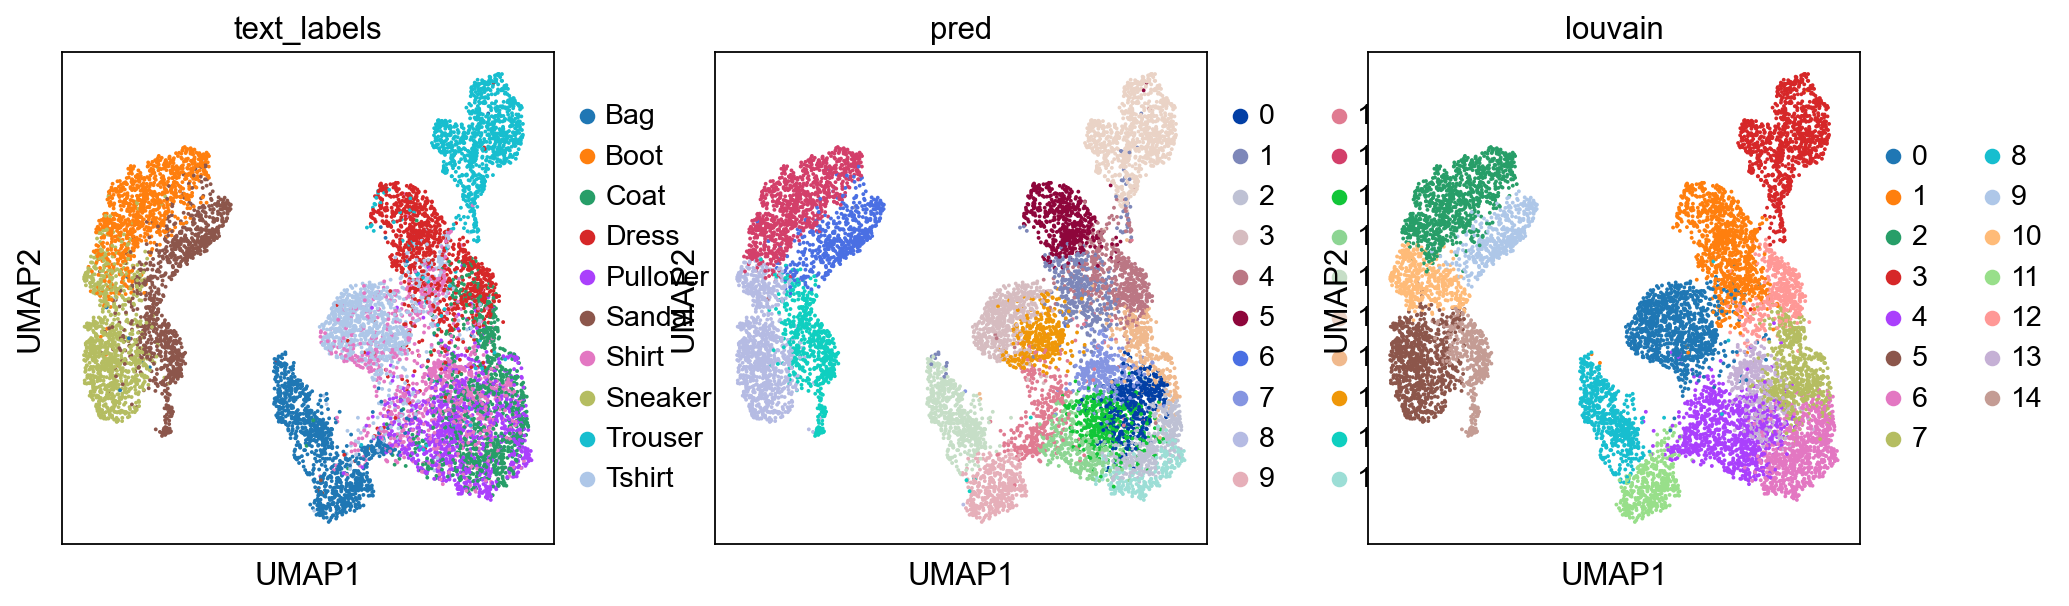
\includegraphics[width=\textwidth]{images/gmmvae_fmnist_us_20c_umap0.png}
%\caption{UMAP (20 components, MNIST)}
%\label{fig:fmnist_us_20c_latent}
%\end{subfigure}
%\begin{subfigure}[b]{0.5\textwidth}
%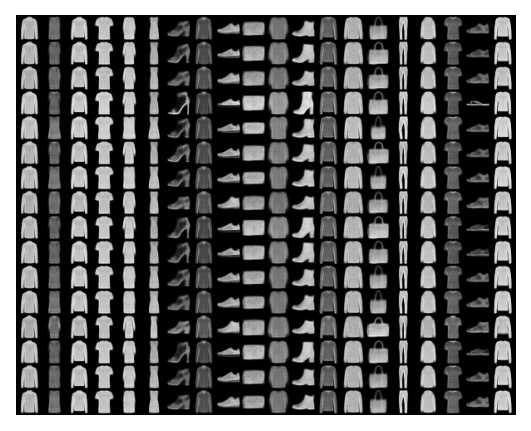
\includegraphics[width=\textwidth]{images/gmmvae_fmnist_us_20c_samples0.png}
%\caption{20 components: generated digits}
%\label{fig:fmnist_us_20c_samples}
%\end{subfigure}
%\caption{GMMVAE with 20 components, unsupervised learning of MNIST.}
%\label{fig:fmnist_us_20}
%\end{figure}

\section{Combination with Louvain clustering}

Louvain clustering achieves accuracy of 0.71 on both the training and the
testing sets.
We supervised trained a GMMVAE and it achieved 0.714 accuracy, an insignificant
difference from Louvain. With further unsupervised training rounds it reached 
0.725 accuracy. Still below the 0.75 we achieved with the best model during 
unsupervised only training but but we were only able to
achieve it with much trying and tuning.
The combination with Louvain is much more consistent as a method.

%Moreover the Louvain clustering on the latent space at least looks nicer than on
%the original space. We didn't have time to confirm this in terms of accuracy.
%If indeed it is the case we could iterate this combined training method with the
%new clusters and see if there is improvement.

\chapter{Tests with PBMCs scRNAseq Data -- Zheng et al}

We first selected a scRNAseq data set~\cite{zheng2017massively} which is easy
because the cells are nicely clustered by cell type.
The main challenge with this data is that it is imbalanced. It has 2623 samples
of 7 cell types overall but in particularly one type (dendritic cells) only has 37 samples.

While Louvain clustering performs well: it achieved 0.93--0.94 accuracy and found 9
clusters, GMMVAE failed to cluster the smallest cell type (see
figure~\ref{fig:zheng_ss_latent}). With the other types
it did ok with accuracy of around 0.92.

\begin{figure}[h]
\centering
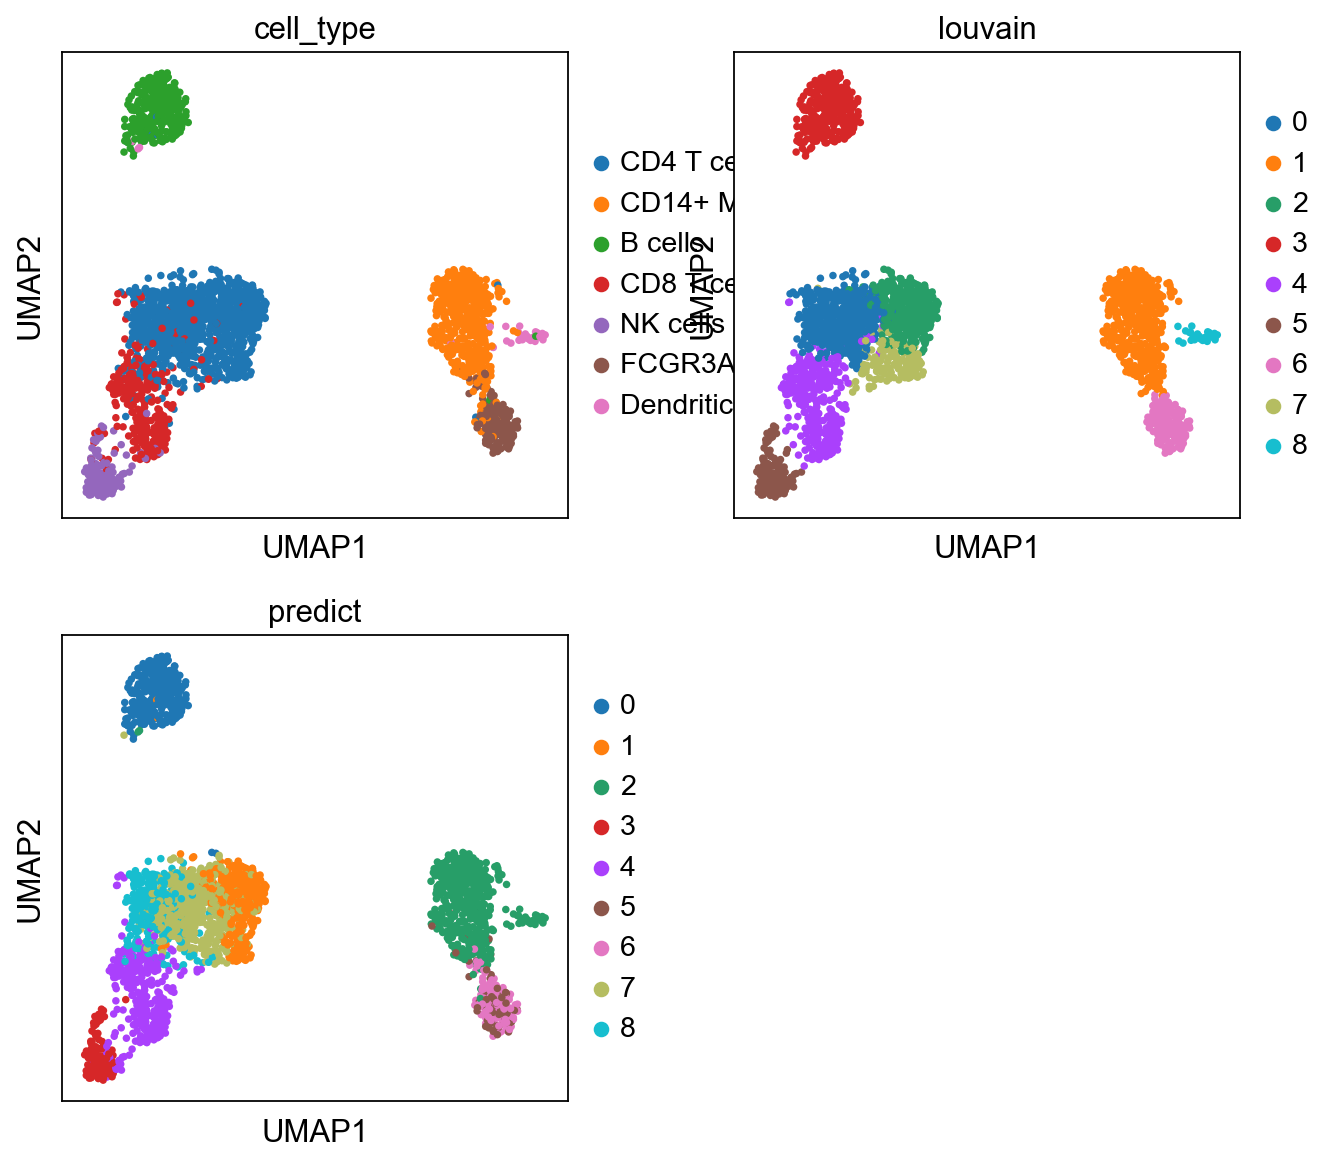
\includegraphics[width=1.1\textwidth]{images/gmmvae_zheng_us_9c_umap.png}
\caption{Zheng dataset, UMAPs. The main issue with GMMVAE is it fails to 
classify the smallest group (Dendritic) in its own cluster.}
\label{fig:zheng_ss_latent}
\end{figure}

In order to overcome this issue we generated a rebalanced data set by selecting 
$300$ samples from each types with repetitions. In addition we added small
Gaussian noise. We also scaled the log-count matrix of the original data set 
so each gene has near standard normal distribution across the samples.

We trained a GMMVAE model by taking turns, first on the rebalanced data, then on
the original data, repeating several times.
We were able to achieve 0.93 accuracy consistently and probably the method can
be a little bit improved by tuning the model and the balancing preprocessing.
In particular it appears that adding the small noise to the rebalanced data
helped the model to learn all the cell types with fewer components.
Figure~\ref{fig:zheng_ss_latent_balanced} visualize with umaps the results 
of this rebalancing method.

\begin{figure}[h]
\centering
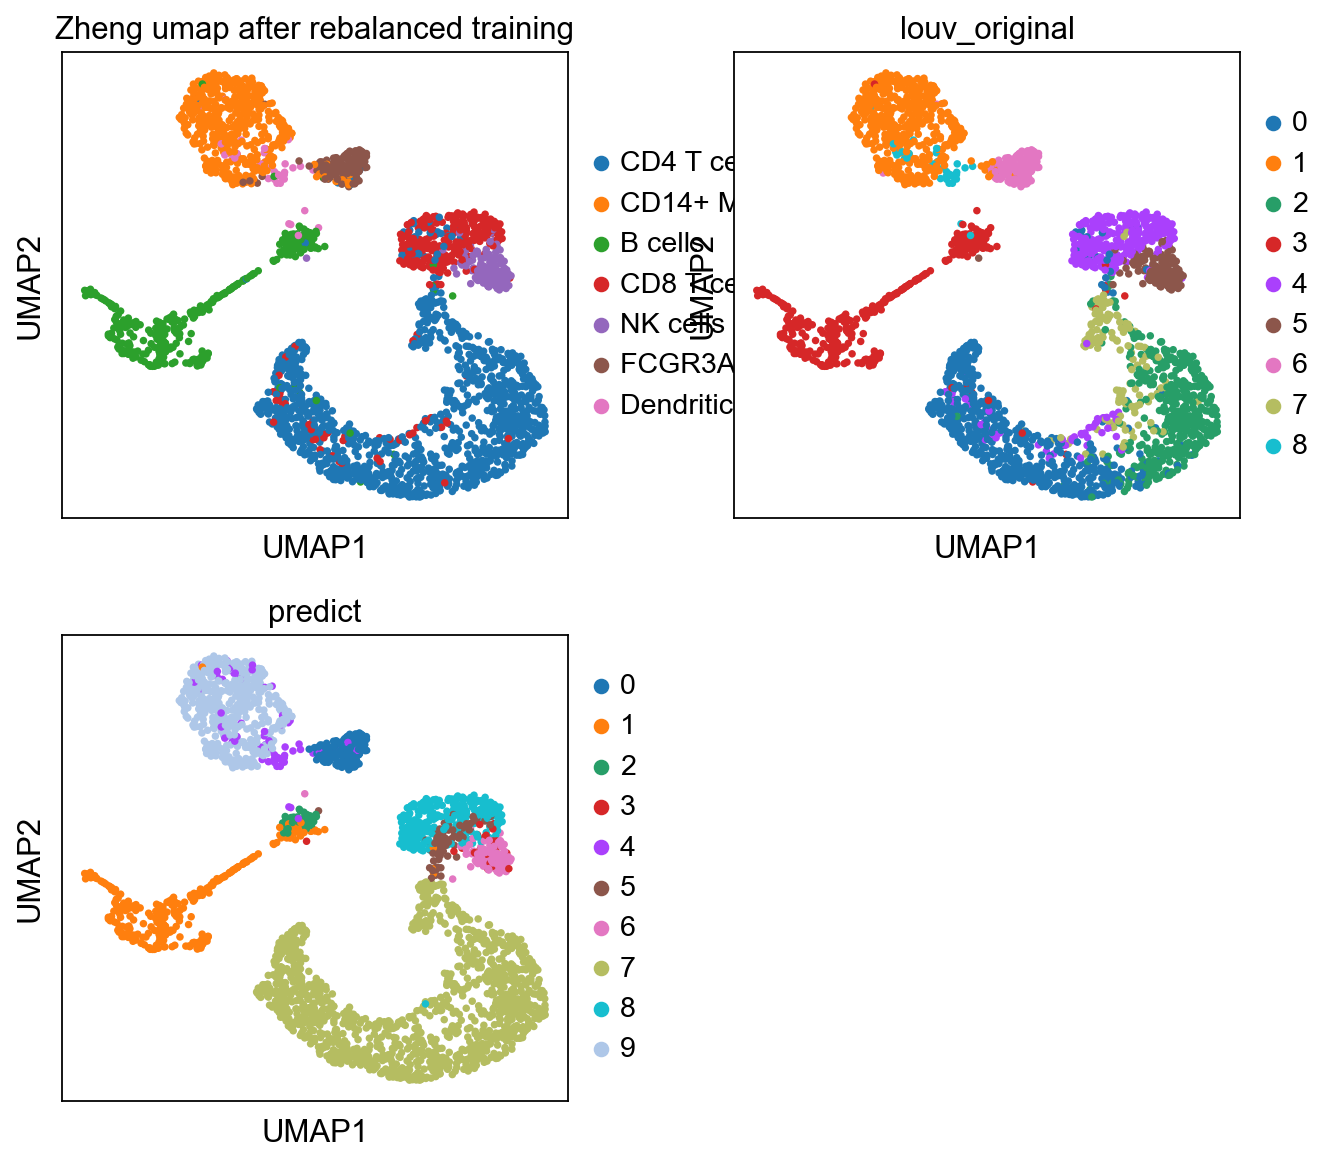
\includegraphics[width=1.1\textwidth]{images/gmmvae_zheng_us_balanced_10c_umap1.png}
\caption{Zheng dataset, UMAPs of the latent space after training 
on the rebalanced and the original data set.
}
\label{fig:zheng_ss_latent_balanced}
\end{figure}


Of course for this particular data it would be easier and faster to use Louvain
clustering and train a GMMVAE model on the clustering if it were needed for some
purpose.
However this experiment gives some insight on the importance of data balancing.

\chapter{Tests with PBMCs scRNAseq Data (Kang et al)}
In these tests we used a scRNAseq dataset~\cite{kang2018multiplexed} of PBMCs
(peripheral blood mononuclear cells) of $7$ cell types which comes from two groups:
control  and treatment. The cells in the treatment group have been exposed to
interferon beta (INF-$\beta$).

Because the data comes from different classes (=cell types) and from two
different batches (control/treatment), 
the conditional version of our mixture model, cDGMMVAE, 
seems to be the most suitable for this type of data. The mixture
components correspond to the cell types, and the condition corresponds to
control/treatment.

\subsection{Unsupervised learning}



\chapter{Discussion, some remarks and conclusions}
punkt.
punkt.
punkt.



\begin{figure}[h]
%\begin{framed}
\centering
\begin{subfigure}[b]{0.9\textwidth}
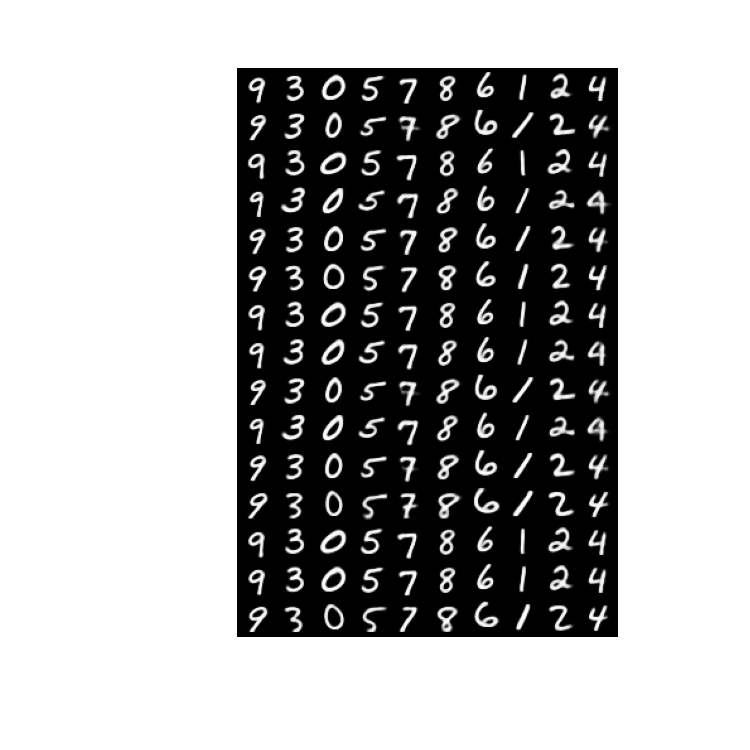
\includegraphics[width=\textwidth]{images/model_mnist_10c_generation.png}
\caption{}
%\caption{blabla}
%\label{bla}
\end{subfigure}
%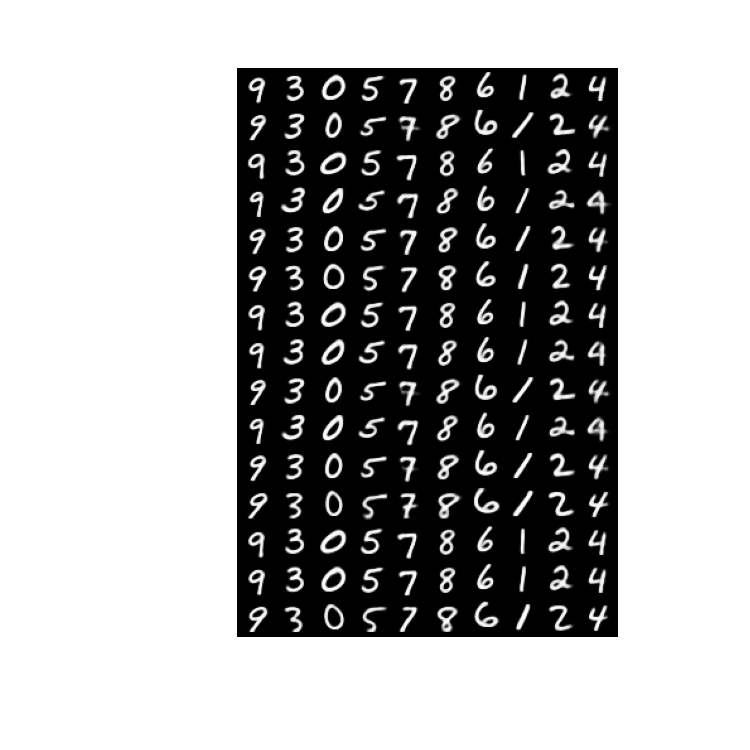
\includegraphics[width=0.4\linewidth]{images/model_mnist_10c_generation.png}
\begin{subfigure}[b]{0.3\textwidth}
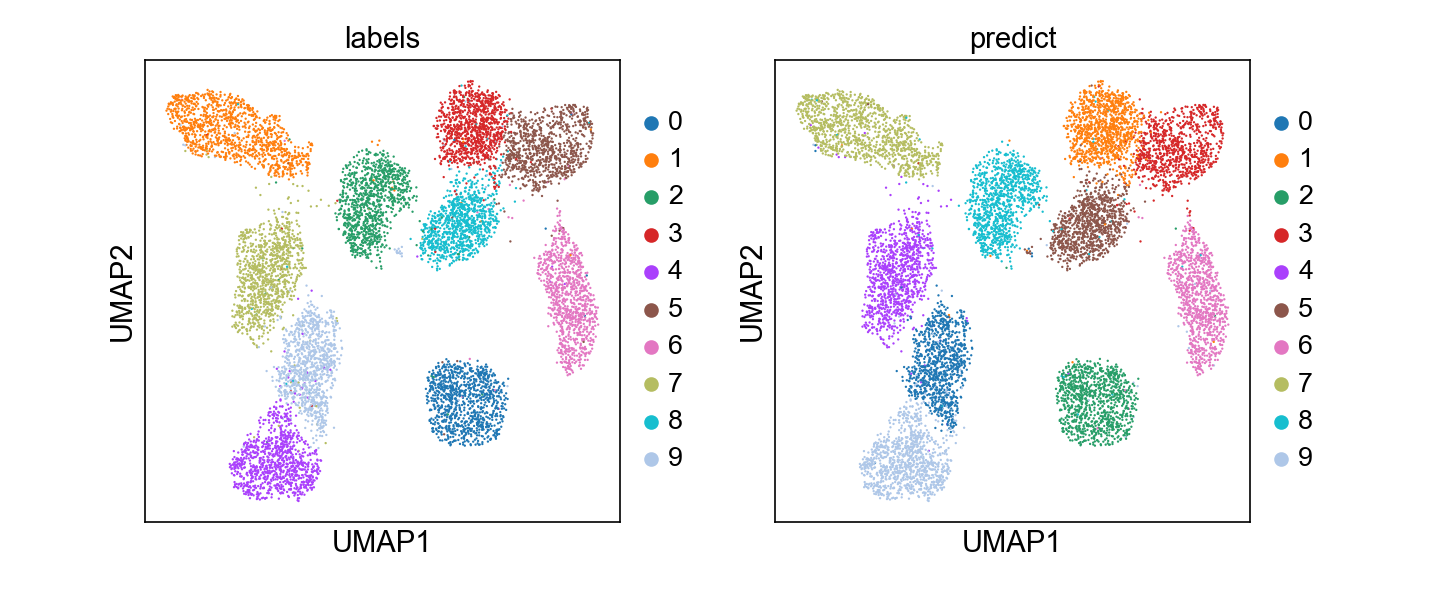
\includegraphics[width=\textwidth]{images/model_mnist_10c_umap.png}
\caption{}
%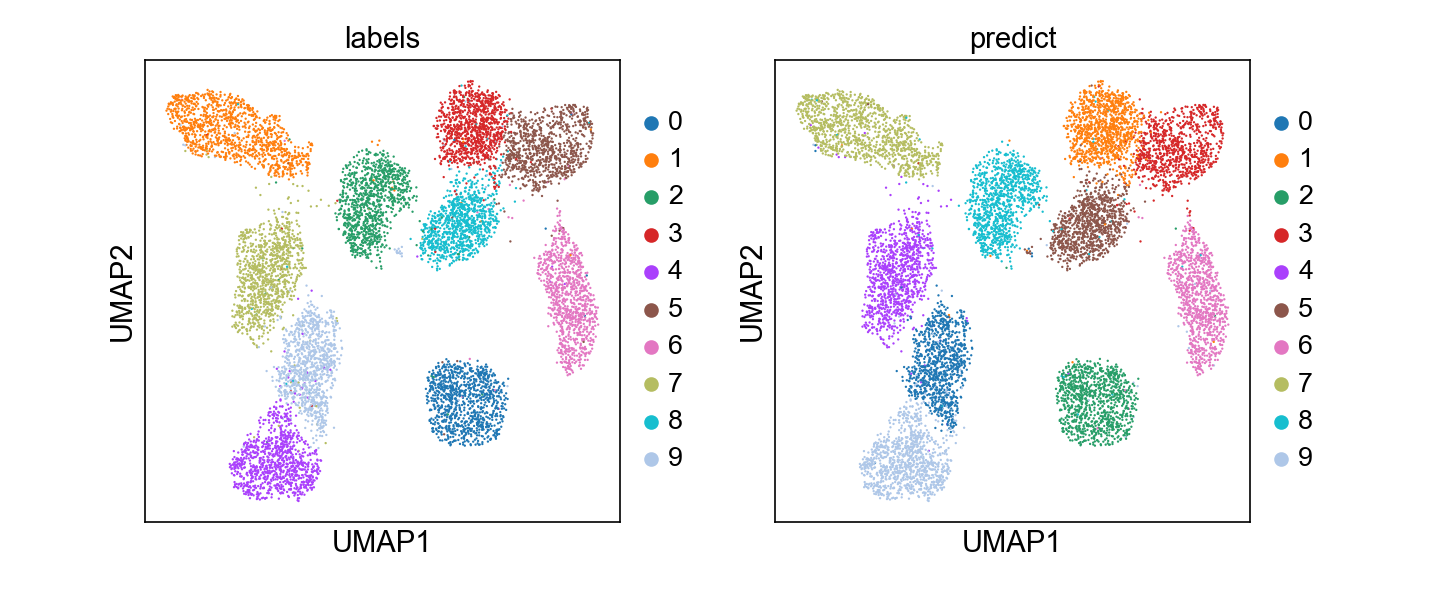
\includegraphics[width=0.4\linewidth]{images/model_mnist_10c_umap.png}
\end{subfigure}
\caption{a figure}
\label{fig:myfig}
%\end{framed}
\end{figure}



%\author{Yiftach Kolb}
%\date{Berlin, \today}
%\maketitle

%\section*{Intro Foo}
%\lipsum{1}
%\section{Bar}
%\lipsum{2}
%\appendix
%\section{Spam}
%\lipsum{3}

\printbibliography

\end{document}


